\documentclass[a4paper, 12pt]{article}
\usepackage[OT1]{fontenc}
\usepackage{bibgerm}
\usepackage{ngerman}
\usepackage[latin1]{inputenc}
\usepackage{graphics}
\usepackage{fancyhdr}
\usepackage{epsfig}
\usepackage{abstract}
% nur f�r linux's pdflatex
%\usepackage{pdfpages}

\begin{document}

%definitionen
\newenvironment{code}
	{\begin{tabbing}}
	{\end{tabbing}}
	
\newcommand{\listitem}[1]{\item \textbf{#1}\\}
\newcommand{\quellcode}[1]{{\em #1}}

% Kopfzeile mit Kapitel
\renewcommand{\sectionmark}[1]{\markleft{#1}{}}
\pagestyle{fancyplain}
\rhead{\footnotesize\thepage}
\lhead{\footnotesize\leftmark}
\cfoot{}

%Titelseite
\begin{titlepage}
\title{
\includegraphics[width=7cm]{../res/uniol.jpg}\\ \vspace{2cm}				
			\textbf{Entwicklung eines Frameworks zur Simulation komponentenbasierter Software-Architekturen\\}
			\vspace{1cm}			 	
			{ \large Individuelles Projekt\\ \vspace{2cm}}}
			
\author{Marko Hoyer\\Hans-Fleischer Stra�e 29-31\\26133 Oldenburg\\
				Marko.Hoyer@informatik.uni-oldenburg.de
				}

\maketitle

\vspace{2cm}
\textbf{Betreuer: } \parbox[t]{7cm}{Jun.-Prof. Dr. Ralf Reussner\\Dipl.-Wirtsch.-Inform. Steffen Becker}

\thispagestyle{empty}
\end{titlepage}

\thispagestyle{empty}
The abstract (100-200 Words).
\newpage

%Inhaltsverzeichnis
\small
\tableofcontents
\normalsize

\thispagestyle{empty}
\newpage

\section{Einleitung}
\label{sec:einleitung}

\subsection{Motivationen und Hintergr�nde}
\label{sec:einleitung:motivation}
Soll ein neu zu erstellendes Softwaresystem auf Basis vorhandener Komponenten erstellt werden, so stellt sich h�ufig die Frage nach der Performance des Gesamtsystems. Deren Beantwortung vor der Implementierung ist h�ufig Voraussetzung zur Einhaltung einiger nichtfunktionaler Anforderungen wie zum Beispiel der mittleren Antwortzeit. Werden die Antwortzeiten der Dienste der einzelnen Komponenten als bekannt vorausgesetzt, so gilt es nun, die Antwortzeit des Gesamtsystems mit einer bestimmten Konfiguration dieser Komponenten und ggf. Konnektoren zu ermitteln. Weiterhin ist h�ufig die Aufdeckung von 'Flaschenh�lsen' im System hilfreich, um durch eine gezielt andere Konfiguration der Komponenten die Performance zu erh�hen.
\par
Besteht das System ausschlie�lich aus linear zusammenh�ngenden Komponenten, deren Dienste der Reihe nach von einer ankommenden Anfrage durchlaufen werden, so gestaltet sich die Analyse des Systems recht einfach. Problemf�lle lassen sich anhand der Einzelzeiten identifizieren, und die gesamte Antwortzeit kann durch Addition der Einzelzeiten relativ leicht ermittelt werden.\\
Beinhalteten die Komponenten innerhalb des Systems jedoch Verzweigungen, so m�ssen alle sich ergebenen Pfade einzeln berechnet und mit einer bestimmten Gewichtung gewertet werden.\\
Weiterhin ergibt es sich in Systemen h�ufig, dass bestimmte Dienste einer Komponente von mehreren Diensten des Gesamtsystems ben�tigt werden. Ein Beispiel hierf�r sind Dienste, die Daten aus einer Datenbank auslesen. Hierbei geht die Analyse des Systems �ber die Pfade hinaus. Es m�ssen nun die Antwortzeiten der Dienste der Komponenten dynamisch auf die Anzahl zu einem Zeitpunkt ankommender Anfragen angepasst werden.\\
�bersteigt die mathematisch exakte Analyse des Systems bereits hier die Grenzen des sinnvoll machbaren, so erscheint die exakte Berechnung bei der Verteilung der einzelnen Komponenten auf verschiedene Prozessoren noch komplexer.
\par
An dieser Stelle kann die Simulation ansetzen. Es werden nun nicht mehr die mathematisch exakten Gegebenheiten berechnet, sondern anhand der Simulation eines Modells mit einer bestimmten Ungenauigkeit ermittelt. Weiterhin lassen sich bei der Simulation 'Flaschenh�lse' identifizieren, die bei der mathematischen Berechnung nur schwer zu ermitteln sind. Hierzu kann beispielsweise einfach das Zeitverhalten einer Anfrage Dienst f�r Dienst aufgezeichnet und hinterher ausgewertet werden. Bild \ref{pic:simul} zeigt schematisch eine solche Simulation.

\begin{figure}[ht]
\begin{center}
\fbox{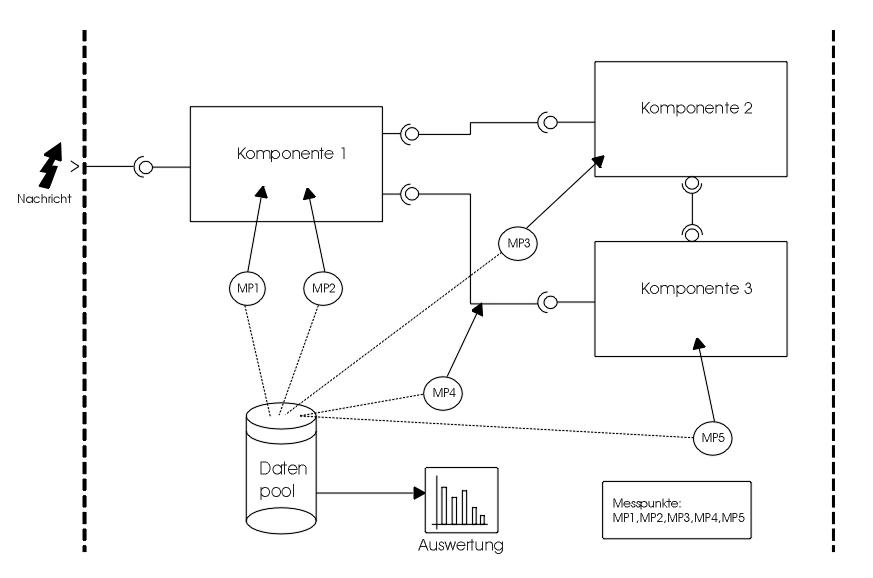
\includegraphics[width=13cm]{../res/simul.jpg}}
\caption{Schematische Darstellung der Simulation}
\label{pic:simul}
\end{center}
\end{figure}

\subsection{Ziele des Individuellen Projektes}
\label{sec:einleitung:ziele}
Ziel dieses Projektes ist die Erstellung einer Infrastruktur f�r die in Abschnitt \ref{sec:einleitung:motivation} erl�uterte Simulation in Form eines Frameworks. Bestandteil des Frameworks wird die Modellierung des Systems und der Komponenten, ein Modell zur Simulation von Anfragen an Dienste des Systems und die Auswertung der gesammelten Daten sein. Diese Bestandteile werden in einer Simulationsumgebung gekapselt.
\par
Bei der Entwicklung wird verst�rkt darauf geachtet, dass kleinere �nderungen und Erweiterungen des Frameworks nicht gro�e �nderungen der Implementierung zur Folge haben. So ist es beispielsweise w�nschenswert, dass einige sich von Modell zu Modell h�ufig �ndernde Bestandteile austauschen lassen, ohne eine Zeile Quellcode des Frameworks �ndern zu m�ssen. Weiterhin sollen Entwurfsentscheidungen, die die Umsetzung einer neuen Modellierung verhindern, �nderbar sein. Das bedeutet, dass die Bestandteile des Frameworks unabh�ngig voneinander austauschbar sein m�ssen.
\par
Das Projekt gliedert sich in die drei im Proposal \cite{lit:proposal} angegebenen Entwicklungsinkremente. Am Ende jedes Inkrementes wird ein der Entwicklungsstufe angepasster Prototyp entstehen, welcher das Framework in seinem aktuellen Stand benutzt.

\subsection{Aufbau dieser Ausarbeitung}
\label{sec:einleitung:aufbau}

Die Ausarbeitung gliedert sich in drei inhaltliche Teile, welche von dieser Einleitung und einem abschlie�enden Fazit eingeschlossen sind.
\par
Der erste Teil befasst sich mit der Kl�rung theoretischer Fragen in Bezug auf die Modellierung von Komponentenarchitekturen und der Simulation. Hierzu werden anf�nglich einige Grundlagen zur Modellierung von Komponenten erarbeitet, welche als Ziel das Modell der gesamten Komponentenarchitektur haben. Darauf aufbauend werden in diesem Modell potentielle Zeitverbraucher identifiziert. Der letzte Teil dieses Kapitels stellt das f�r das Framework entwickelte Simulationsmodell vor.
\par
Der zweite und gleichzeitig gr��te Teil dieser Ausarbeitung ist dem Entwurf des Frameworks gewidmet. Dieser beginnt mit dem Festlegen einiger allgemeiner Anforderungen an das Framework. Der zweite Teil dieses Kapitels erarbeitet eine sinnvolle Architektur des Frameworks. Das bedeutet, dass an dieser Stelle das Framework in seine groben Bestandteile gegliedert wird. Innerhalb dieser Teile werden dann unter Betrachtung von speziellen an den jeweiligen Teil gestellten Anforderungen einzelne Komponenten identifiziert. Der dritte Teil des Entwurfs bildet dann schlie�lich die Architektur mit ihren Komponenten auf Klassen und Pakete ab. Hier werden einige der Entwurfsentscheidungen zum besseren Verst�ndnis des Frameworks detailiert erkl�rt.
\par
Das dritte und abschlie�ende inhaltliche Kapitel der Ausarbeitung geht auf die Anwendung des Frameworks ein. Hierzu wird anhand eines Beispiels die Benutzung der Basisfunktionalit�t beschrieben. Weiterhin wird auf die Erweiterungsm�glichkeiten und deren Ansatzpunkte im Framework eingegangen. Um den Umfang der Funktionalit�t des Frameworks einsch�tzen zu k�nnen, wird dem Leser abschlie�end ein �berblick �ber die Grenzen des Frameworks vermittelt.
\newpage

\section{Modellbildung}
\label{sec:modell}
In diesem Kapitel wird auf die Entwicklung und Auswahl der im Framework verwendeten Modelle eingegangen. Hierzu geh�rt die Abbildung der Komponenten und der Architektur in ein Modell, die Identifizierung der Zeitverbraucher innerhalb der Architektur und die darauf aufbauende Modellierung der eigendlichen Simulation.

\subsection{Grundlagen zur Modellierung von Komponenten und Komponentenarchitekturen}
\label{sec:modell:grundlagen}
Da sich dieses Framework mit der Simulation von Modellen von Architekturen und Komponenten befassen soll, gilt es als erstes, geeignete Modelle f�r die Komponenten und die Architektur auszuw�hlen und diese ggf. f�r die Simulation anzupassen. Als Basis hierf�r wird auf ein Komponentenmodell zur�ckgegriffen, welches in \cite{lit:reussner01} vorgestellt wird. In diesem Modell repr�sentieren sich Komponenten durch eine Reihe angebotener Dienste. Diese Dienste werden nach au�en hin durch Schnittstellen (in \cite{lit:reussner01} als {\em Angebotssschnittstellen} bezeichnet) abgebildet. Die Dienste selber k�nnen andere m�glicherweise externe Dienste zu ihrer Ausf�hrung ben�tigen, welche ebenso durch Schnittstellen (in \cite{lit:reussner01} als {\em Bedarfsschnittstelle} bezeichnet) nach au�en abgebildet werden.

\subsubsection{Auswahl des Schnittstellenmodells}
\label{sec:modell:grundlagen:schnittstellen}
Das Modell sieht je nach Anfordung unterschiedliche Schnittstellenmodelle vor, welche hierarchisch angeordnet sind. Die aus \cite{lit:reussner01} entnommene Auflistung erl�utert diese kurz.
\begin{itemize}
\item \textbf{Signaturlisten} beschreiben die Signaturen von Diensten. Dazu geh�ren Name, Parameterzahl, Parametertypen und ggf. der R�ckgabetyp des Dienstes
\item \textbf{Protokolle} spezifizieren Reihenfolgen von Dienstaufrufen. Damit wird die Verf�gbarkeit von Diensten einer Komponente in Abh�ngigkeit ihres internen Zustands beschrieben sowie die Reihenfolgen, mit denen die Komponente externe Dienste aufrufen kann.

\item \textbf{Qualit�tsattribute und Nicht-funktionale Eigenschaften} betreffen Randbedingungen, die spezifizieren wie eine Komponente ihre Funktionalit�t erf�llt. Solche Randbedingungen betreffen beispielsweise Zuverl�ssigkeit, Effizienz bestimmter Dienste oder Robustheit.

\end{itemize}

Da im Framework die Komponenten nicht als Blackboxes simuliert werden sollen, ben�tigen die Schnittstellen selber keine Beschreibung der Nicht-funktionalen Eigenschaften der Komponente. Diese werden, wie in Abschnitt \ref{sec:modell:bestandteile} erl�utert, direkt im Modell der Dienste der Komponenten umgesetzt. Auf die Modellierung von Protokollen kann ebenfalls verzichtet werden, da die Simulation nicht dazu dient, Interoperabilit�t zu pr�fen. Es wird bereits davon ausgegangen, dass die Komponenten der zu simulierenden Architektur zusammenpassen. Somit gen�gt es, die unterste Ebene der Schnittstellenmodelle, die Signaturlisten, zu verwenden.


\subsubsection{Modellierung der Dienste}
\label{sec:modell:grundlagen:dienste}
Die Dienste einer Komponente werden in \cite{lit:reussner01} durch endliche Automaten (dort {\em Dienstbedarfautomaten} genannt) umgesetzt, wobei die Zust�nde einen Kontrollfluss unabh�ngig von anderen Diensten repr�sentieren und die Transitionen die Aufrufe anderer m�glicherweise externer Dienste darstellen. Ist ein Zustand als Endzustand definiert, so wird dies als Beendigung eines Dienstes (durch Erfolg oder Ausnahme) gewertet. Verlassen zwei Transitonen einen Zustand, so repr�sentiert dieses einen Zweig im Kontrollfluss, welcher in der Simulation durch an den Transitionen befindlichen Wahrscheinlichkeiten aufgel�st wird.
Bild \ref{pic:modell} zeigt einen Dienstbedarfsautomaten (f�r Dienst e0). Dieser k�nnte folgenden Quellcode einer Komponente modellieren.\\
\begin{code}
be\=gi\=n \=e0\=()\\
\>{\em interne Befehle}\\
\>if ({\em Bedingung})\\
\>\>e1();\\
\>\>{\em interne Befehle}\\
\>\>e2();\\
\>else \\
\>\>e3();\\
end e0

\end{code}

\subsubsection{Verbindungen zwischen Komponenten}
\label{sec:modell:grundlagen:verbindung}

Nachdem nun einzelne Komponenten modelliert werden k�nnen, m�ssen jetzt M�glichkeiten geschaffen werden, mehrere dieser Komponenten untereinander oder mit der Aussenwelt zu verbinden. Bei der Verbindung zweier Komponenten untereinander wird eine Bedarfsschnittstelle einer Komponente mit der Angebotsschnittstelle einer anderen verbunden. Bei der Verbindung zur Au�enwelt dagegen werden zwei Bedarfs- bzw. Angebotsschnittstellen miteinander verbunden. Die erste der beiden Verbindungen werden im Folgenden als ComponentMapping und die zweite als ComponentBinding bezeichnet. Abbildung \ref{pic:modell} stellt diesen Unterschied anschaulich dar.
\par
Da Schnittstellen unter Umst�nden mehrere Dienste kapseln, m�ssen innerhalb einer dieser Verbindungen Strukturen zur Verf�gung stehen, die jeden einzelnen Dienst verbinden. Diese Einzelverbindungen werden im Folgenden als Mapping bzw. Binding bezeichnet.

\begin{figure}[ht]
\begin{center}
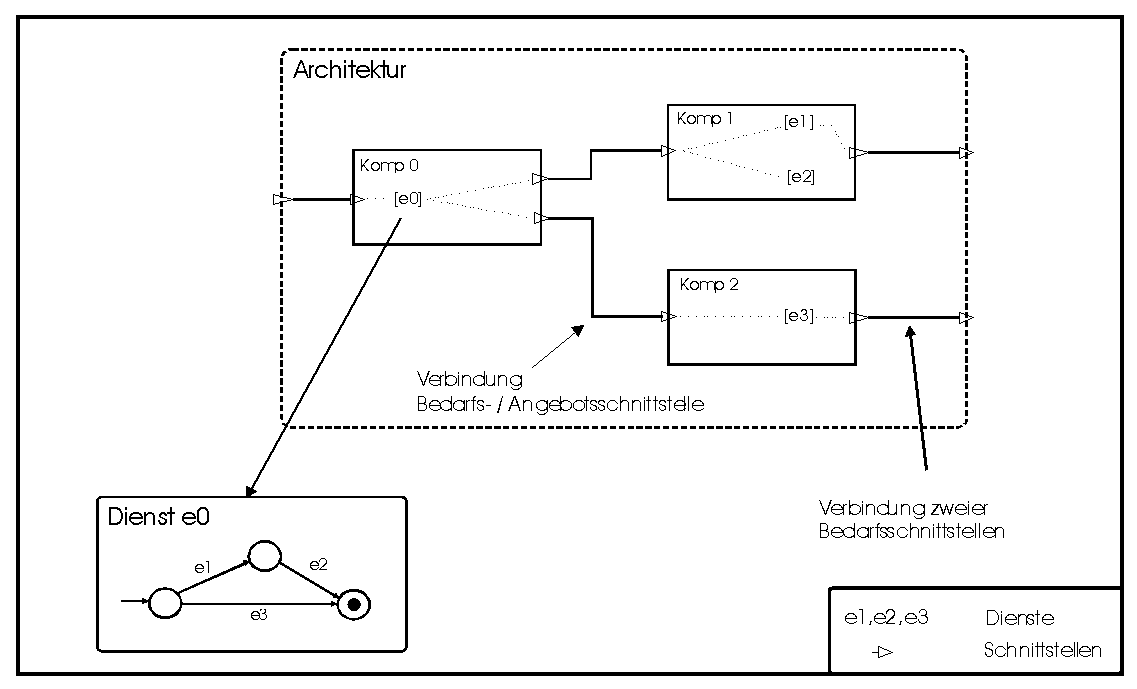
\includegraphics[width=13.5cm]{../res/modell.png}
\caption{Modell einer Komponentenarchitektur}
\label{pic:modell}
\end{center}
\end{figure}


\subsection{Identifizierung von zeitverbrauchenden Bestandteilen des Modells}
\label{sec:modell:bestandteile}
Nachdem im vorherigen Abschnitt die Modellierung einer Komponente beschrieben wurde, m�ssen nun innerhalb des Modells Zeitverbraucher identifiziert werden, welche der Simulation sp�ter als Datenbasis dienen werden. Hierzu hangeln wir uns im Modell durch den Kontrollfluss einer Anfrage.
\par
Dieser beginnt f�r gew�hnlich am Rand einer Architektur durch den Aufruf eines Dienstes, welcher �ber ein Binding innerhalb eines ComponentBinding in einer Komponente erreichbar ist. Ist diese �ber z.B. einen Softwarebus erreichbar, ergibt sich hier ein m�glichweise sogar dynamischer Zeitverbraucher. Es ist davon auszugehen, das alle Bindings innerhalb eines ComponentBinding die gleichen Laufzeiteigenschaften haben, da ein ComponentBinding ein Interface repr�sentiert und dieses f�r alle dort deklarierten Dienste den gleichen Weg nehmen wird. Somit gibt ein ComponentBinding eine dynamische Zeit vor, die alle enthaltenen Bindings benutzen k�nnen. Ebenso wie bei ComponentBindings verh�lt es sich bei der Verbindung zweier Komponenten, also bei ComponentMappings.
\par
Erreicht die Anfrage das Angebotsinterface, steht ihr als n�chstes der Weg zum Dienstbedarfsautomat bevor. Hierbei handelt es sich jedoch um einen Weg, welcher �blicherweise nur im Modell existiert. In der Realit�t ist ein Dienst f�r gew�hnlich eine Implementierung einer Methode eines Interface. Somit ist dieser Weg kein Zeitverbraucher. Soll trotzdem an dieser Stelle eine Zeitverz�gerung modelliert werden, so ist es prinzipiell m�glich, diese in den  Dienst einzurechnen.
\par
Dienste werden, wie in Abschnitt \ref{sec:modell:grundlagen:dienste} beschrieben, durch Dienstbedarfsautomaten also endliche Automaten modelliert, wobei Zust�nde interne Befehle und Transitionen externe Dienste repr�sentieren. Interne Befehle ben�tigen Rechenzeit, die sich auch wieder dynamisch �ndern kann, kommen also als dynamische Zeitverbraucher in Betracht. Externe Dienstaufrufe sind keine direkten Zeitverbaucher. Ihre Zeit berechnet sich aus dem Zeitverbauch des aufzurufenden Dienstes und dem Weg dahin.
\par
Nachdem nun alle Zeitverbraucher entlang dem Kontrollfluss einer Anfrage identifiziert wurden, besch�ftigt sich der n�chste Abschnitt mit dem Aufbau eines Simulationsmodells.

\subsection{Aufbau des Simulationsmodells}
\label{sec:modell:simulation}

Beim Entwurf des Simulationsmodell geht es darum, an die Architektur gestellte Anfragen und deren Wechselwirkungen innerhalb der Architektur m�glichst realit�tsnah zu simulieren. Es kommen grunds�tzlich zwei M�glichkeiten in Frage, die im n�chsten Abschnitt kurz diskutiert werden.

\subsubsection{Reelle Threads vs. simulierte Threads}
\label{sec:modell:simulation:reellvssim}

Bei der Simulation mit reellen Threads wird f�r jede Anfrage an das System ein reelles Thread erzeugt. Wie in der Realit�t auch, werden diese an bestimmten Stellen in der Architektur Zeit verbrauchen. Dies l��t sich erreichen, indem die Threads an diesen Stellen f�r eine bestimmte Zeit blockiert werden. Diese Zeit kann im einfachsten Fall der Realit�t entsprechen, was dazu f�hrt, dass das Modell in Echtzeit arbeitet. Nachteile bei dieser Methode ergeben sich, wenn sowohl kurze als auch lange Verz�gerungszeiten in der Architektur auftreten, da sich dann m�glicherweise eine unn�tige Wartezeit ergibt. Diese k�nnte man �berbr�cken, indem die Simulationszeit gezielt  vorgestellt wird. Als erheblicher Nachteil bei diesem Prinzip erweist sich jedoch die Sychronisation der einzelnen Threads insbesondere wenn sie gleichzeitig an der selben Stelle auftreten. Experimentelle Versuche erwiesen hier aufgrund eben genannter Problematik komplizierte schlecht erweiterbare Konstrukte. Aufgrund dieser Nachteile, insbesondere der Synchronisationsproblematik, wird von der Verwendung dieses Ansatzes abgesehen. 
\par
Der zweite Ansatz simuliert Threads. Hierzu werden Stellen innerhalb der Architektur mit einer Zeit markiert. Die simulierten Threads starten an einer dieser Stellen und addieren dann die Zeiten entlang ihres Kontrollflusses auf. Somit wird die Zeit der Simulation unabh�ngig von der Architektur, da die zu verbrauchende Zeit nicht verstreichen muss. Dieser Ansatz gestattet problemlos die Verarbeitung mehrer Anfragen, solange der Durchlauf einer Anfrage keinerlei Einfluss auf den  Kontrollfluss oder die zeitverbrauchenden Bestandteile der Architektur mit sich bringt. Ein solches Modell spiegelt jedoch die Realit�t nicht gut wieder. Es ist beispielsweise w�nschenswert, bei der Modulation einer Single-Thread-Komponente die Wartezeit einer Anfrage zu erh�hen, wenn gerade eine andere Anfrage verarbeitet wird. Auf diese Art lassen sich ebenfalls Auslastungen des Prozessors, auf dem die Komponente l�uft, modellieren. Weiterhin sinnvoll erscheint die dynamische �nderung des Kontrollflusses. Folgendes Beispiel erl�utert den Sinn dieser Modellierung.
\par
Soll das Modell eine Schleife im Kontrollfluss modellieren, so benutzt man folgenden Ansatz. Man modelliert wie in Bild \ref{pic:rekurs} dargestellt eine Endlosschleife, wobei 1.0 und 0.0 die, wie in Kapitel  \ref{sec:modell:grundlagen:dienste} beschrieben, Wahrscheinlichkeiten zur Aufl�sung des Zweiges darstellen. Soll die Schleife nach einigen Durchl�ufen abgebrochen werden, so m�ssen diese Wahrscheinlichkeiten in Abh�ngigkeit der Anzahl der Durchl�ufe ver�ndert werden, damit die Schleife verlassen wird.

\begin{figure}[ht]
\begin{center}
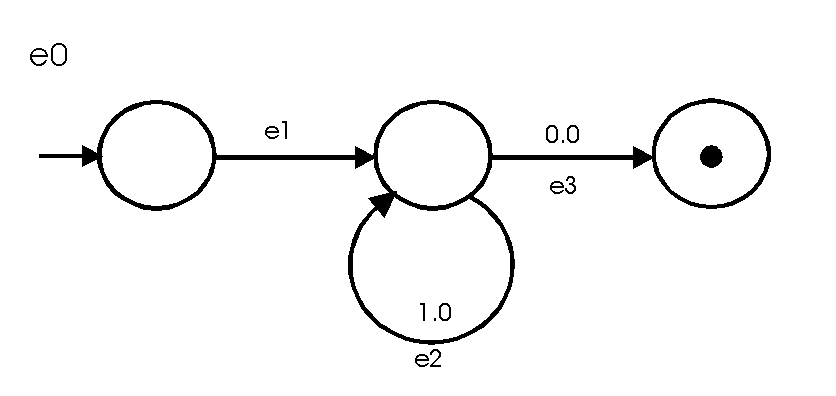
\includegraphics[width=7cm]{../res/rekurs.png}
\caption{Dienstbedarfsautomat moduliert eine Endlosschleife}
\label{pic:rekurs}
\end{center}
\end{figure}

Um diese beiden Anforderungen im Simualtionsmodell unterzubringen, ist auch in diesem Fall die Synchronisation der Anfragen untereinander notwendig, damit diese ihren gleichzeitigen Aufenthalt an ein und der selben Stelle in der Architektur �berhaupt wahrnehmen k�nnen. Hierbei kommt man schnell zu der Erkenntnis, dass das einfache aufaddieren der Zeiten hier nicht mehr gen�gt, da das Einrechnen der Wechselwirkungen durch andere Threads unm�glich ist. Eine kleine Modifikation des Ansatzes l�st dieses Problem. Die Simulation wird pro Anfrage nicht mehr am St�ck durchgef�hrt, sondern Schrittweise. Dies bedeutet, dass alle zur Zeit vorhandenen Anfragen um die gleiche Schrittweite vorgestellt werden. Nun ist die dynamische Anpassung der Wartezeiten problemlos m�glich, da alle Anfrage quasi gleichzeitig simuliert werden. Die maximale Schrittweite eines Schrittes ist hierbei begrenzt durch die Zeit, in der keines der Threads eine Zustands�nderung erf�hrt. Mit Zustands�nderung sei hier der Wechsel eines Threads zum n�chsten zeitverbrauchenden Bestandteil der Architektur im Kontrollfluss gemeint. Der folgende Abschnitt verdeutlicht die Umsetzung dieses Ansatzes anhand eines Beispiels.

\subsubsection{Ablauf einer Simulation}
\label{sec:modell:simulation:sync}

In Bild \ref{pic:ablauf} ist eine m�gliche Startkonfiguration einer Simulation dargestellt. Es befinden sich zum Zeitpunkt 0 drei Anfragen an bestimmten Punkten des Systems. Entlang der Zeitachse t sind f�r jedes Thread die Wartezeiten eingetragen, welche hier der Einfachheit halber statisch gew�hlt sind. 

\begin{figure}[ht]
\begin{center}
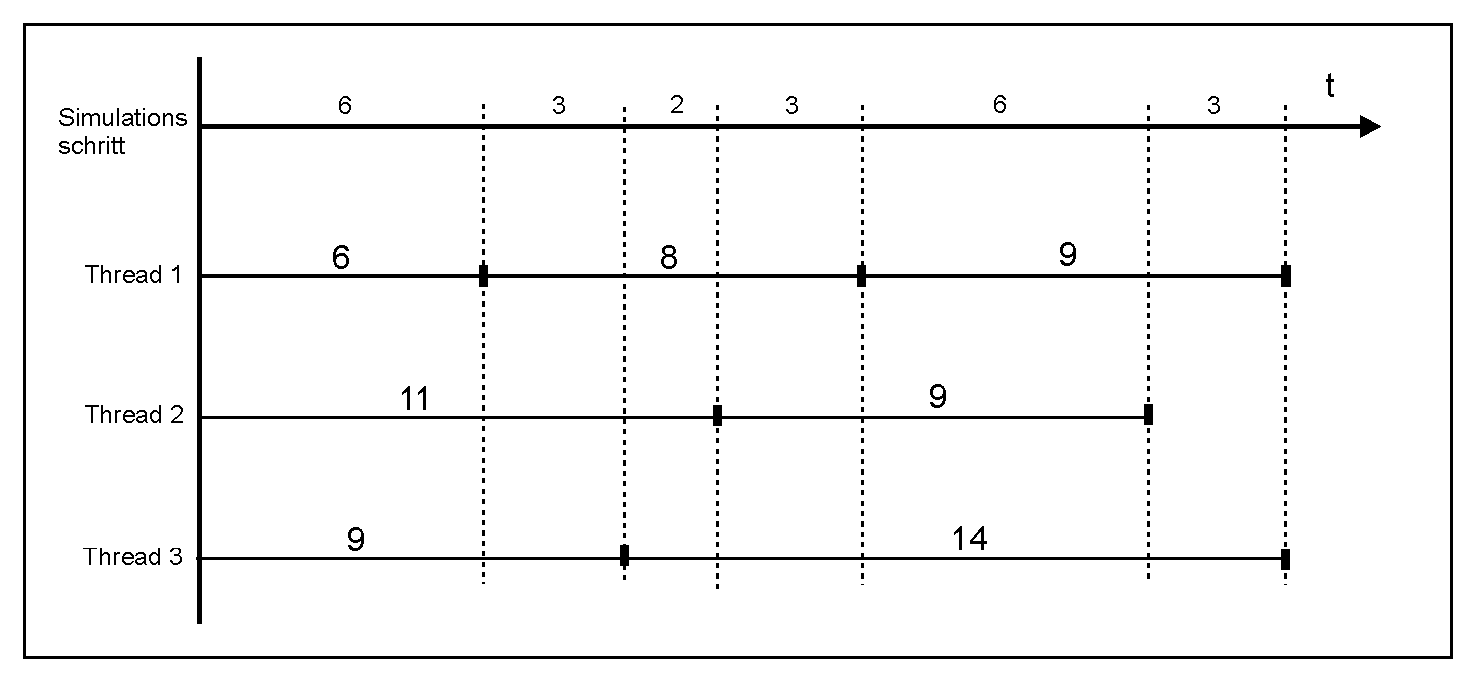
\includegraphics[width=13cm]{../res/simmodell.png}
\caption{Simulation von Anfragen}
\label{pic:ablauf}
\end{center}
\end{figure}

Der n�chste Zeitschritt berechnet sich aus der k�rzesten noch verbleibenden Wartezeit aller Threads, im Beispiel also 6, da nach Ablauf dieser Zeit Thread 1 seinen Zustand �ndert. Wird der Zeitschritt ausgef�hrt, so verringert sich bei allen Threads die verbleibende Zeit um diesen Schritt. Erreicht ein Thread eine verbleibende Zeit von 0, so wechselt dieses zu seinem n�chsten Zeitverbraucher im Kontrollfluss. Existiert dieser nicht, so hat das Thread die Abarbeitung der Anfrage beendet. In Bild \ref{pic:ablauf} erreicht beispielsweise Thread 2 diesen Zustand nach 20 Zeiteinheiten. Nachdem alle Threads diesen Zustand erreicht haben, im Beispiel nach 23 Zeiteinheiten, endet die Simulation.\\

\par
Nachdem in diesem Kapitel die theoretischen Hintergr�nde f�r die Simulation von Komponentarchitekturen ausgibig diskutiert wurden, befasst sich das n�chste Kapitel mit der praktischen Umsetzung dieser Modelle.
\newpage

\section{Entwurf}
\label{sec:entwurf}
Nachdem im vorherigen Kapitel die theoretischen Hintergr�nde der Anwendungsdom�ne des Frameworks diskutiert und die ben�tigten Modelle ausgearbeitet wurden, befasst sich dieser Teil der Ausarbeitung mit der praktischen Umsetzung. Hierf�r werden anfangs die Anforderungen an das Framework ermittelt. Anschlie�end wird es in seine groben Bestandteile gegliedert, welche dann einzeln analysiert und abschlie�end im Feinentwurf auf die implementierenden Klassen und Interfaces abgebildet werden.

\subsection{Anforderungen}
\label{sec:entwurf:anf}

Das Gebiet der Simulation von Komponentenarchitekturen ist z.Z. wenig erforscht. Dieses Framework bildet den Versuch der Umsetzung einer Simulationsumgebung, ohne auf bereits bew�hrte Methoden auf diesem Gebiet zur�ckgreifen zu k�nnen. Hierbei ergeben sich zwei allgemeine funktionale Anforderungen an das Framework selber, welche im Folgenden erl�utert werden. Auf spezielle Anforderungen an die Komponenten des Frameworks wird bei der genaueren Analyse seiner Einzelteile in Kapitel \ref{sec:entwurf:grob} eingegangen.

\subsubsection{Bereitstellung von Basisfunktionalit�ten}
\label{sec:entwurf:anf:basis}
Das Framework soll in allen im Folgenden erl�uterten Bereichen zusammen lauff�hige Basisfunktionalit�ten bieten. Dies kann zum einen f�r den unver�nderten Gebrauch notwendig sein, wobei dann ohne weitere Implementierungen Simulationen auf dem Framework ausgef�hrt werden k�nnen. Wichtiger in diesem Zusammenhang erscheint jedoch die gezielte Erweiterung an bestimmten Stellen des Frameworks, wobei andere Bereiche unver�ndert genutzt werden k�nnen. Die zu unterst�tzenden Bereiche der Simulationsumgebung lassen sich grob in drei Teile aufspalten. 

\begin{itemize}

\listitem{Modellierung einer Komponentenarchitektur}
Dieser Teil sorgt f�r die Umsetzung des in Kapitel \ref{sec:modell:grundlagen} vorgestellten Komponentenmodells. Hierbei gilt es, den Aufbau eines Architekturmodells in einem f�r die Simulation nutzbaren Format zu erm�glichen.
	
\listitem{Simulation von Anfragen}
Im zweiten Teil geht es um die Simulation von Anfragen an das mit dem ersten Teil aufgebaute Modell. Hierzu soll das Simulationsmodell aus Kapitel \ref{sec:modell:simulation} umgesetzt werden. 

\listitem{Erfassung von Simulationsdaten}
Hier sollen die w�hrend der Simulation enstandenen Daten gesammelt werden. Bei der Implementierung der Basisfunktionalit�t gen�gt es, Daten nach der Simulation auswerten zu k�nnen. Um jedoch auch w�hrend der Simulation Analysen vornehmen zu k�nnen, soll dieser Teil die M�glichkeit offen lassen, Daten auch direkt auswerten zu k�nnen.
\end{itemize}
	
\subsubsection{M�glichkeiten zum Austausch und zur Erweiterbarkeit}
\label{sec:entwurf:anf:erweit}

Aufgrund der oben angesprochenen Problematik ist beim Entwurf des Frame\-works darauf zu achten, dass es m�glichst modular aufgebaut ist. Das bedeutet, es m�ssen sich alle gr��eren Bestandteile des Frameworks austauschen lassen, ohne die Funktionalit�t anderer Bereiche ebenfalls �ndern zu m�ssen. So ist es beispielsweise w�nschenswert, den Teil f�r die Modellierung auf ein anderes Komponentenmodell umstellen und mit diesem die Funktionalit�t des Simulations- und des Auswertungsteils verwenden zu k�nnen.
\par
Weiterhin sollen die Basisimplementierungen nicht nur ausschlie�lich austauschbare Referenzimplementierungen sein, sondern auch die M�glichkeit der Erweiterung offen lassen.  

\subsection{Architektur des Frameworks}
\label{sec:entwurf:grob}

Wie in Kapitel \ref{sec:entwurf:anf:basis} erl�utert, teilt sich das Framework in drei Bestandteile: das Modell, die Simulation und die Auswertung. Um diese Teile bereits in der Architekturebene m�glichst unabh�ngig und damit austauschbar zu gestalten, werden Verbindungen dieser Ebenen untereinander nur �ber eine vierte �bergeordnete Ebene zugelassen. Diese Ebene wird im Folgenden als {\em Simulationsumgebung} oder {\em simulation environment} bezeichnet. Abbildung \ref{pic:architecture} verdeutlicht diesen Zusammenhang. Weiterhin zeigt diese Abbildung (gestrichelt gezeichnet) eine Reihe von Erweiterungsm�glichkeiten und die Positionen, an denen sie ansetzen.

\begin{figure}[ht]
\begin{center}
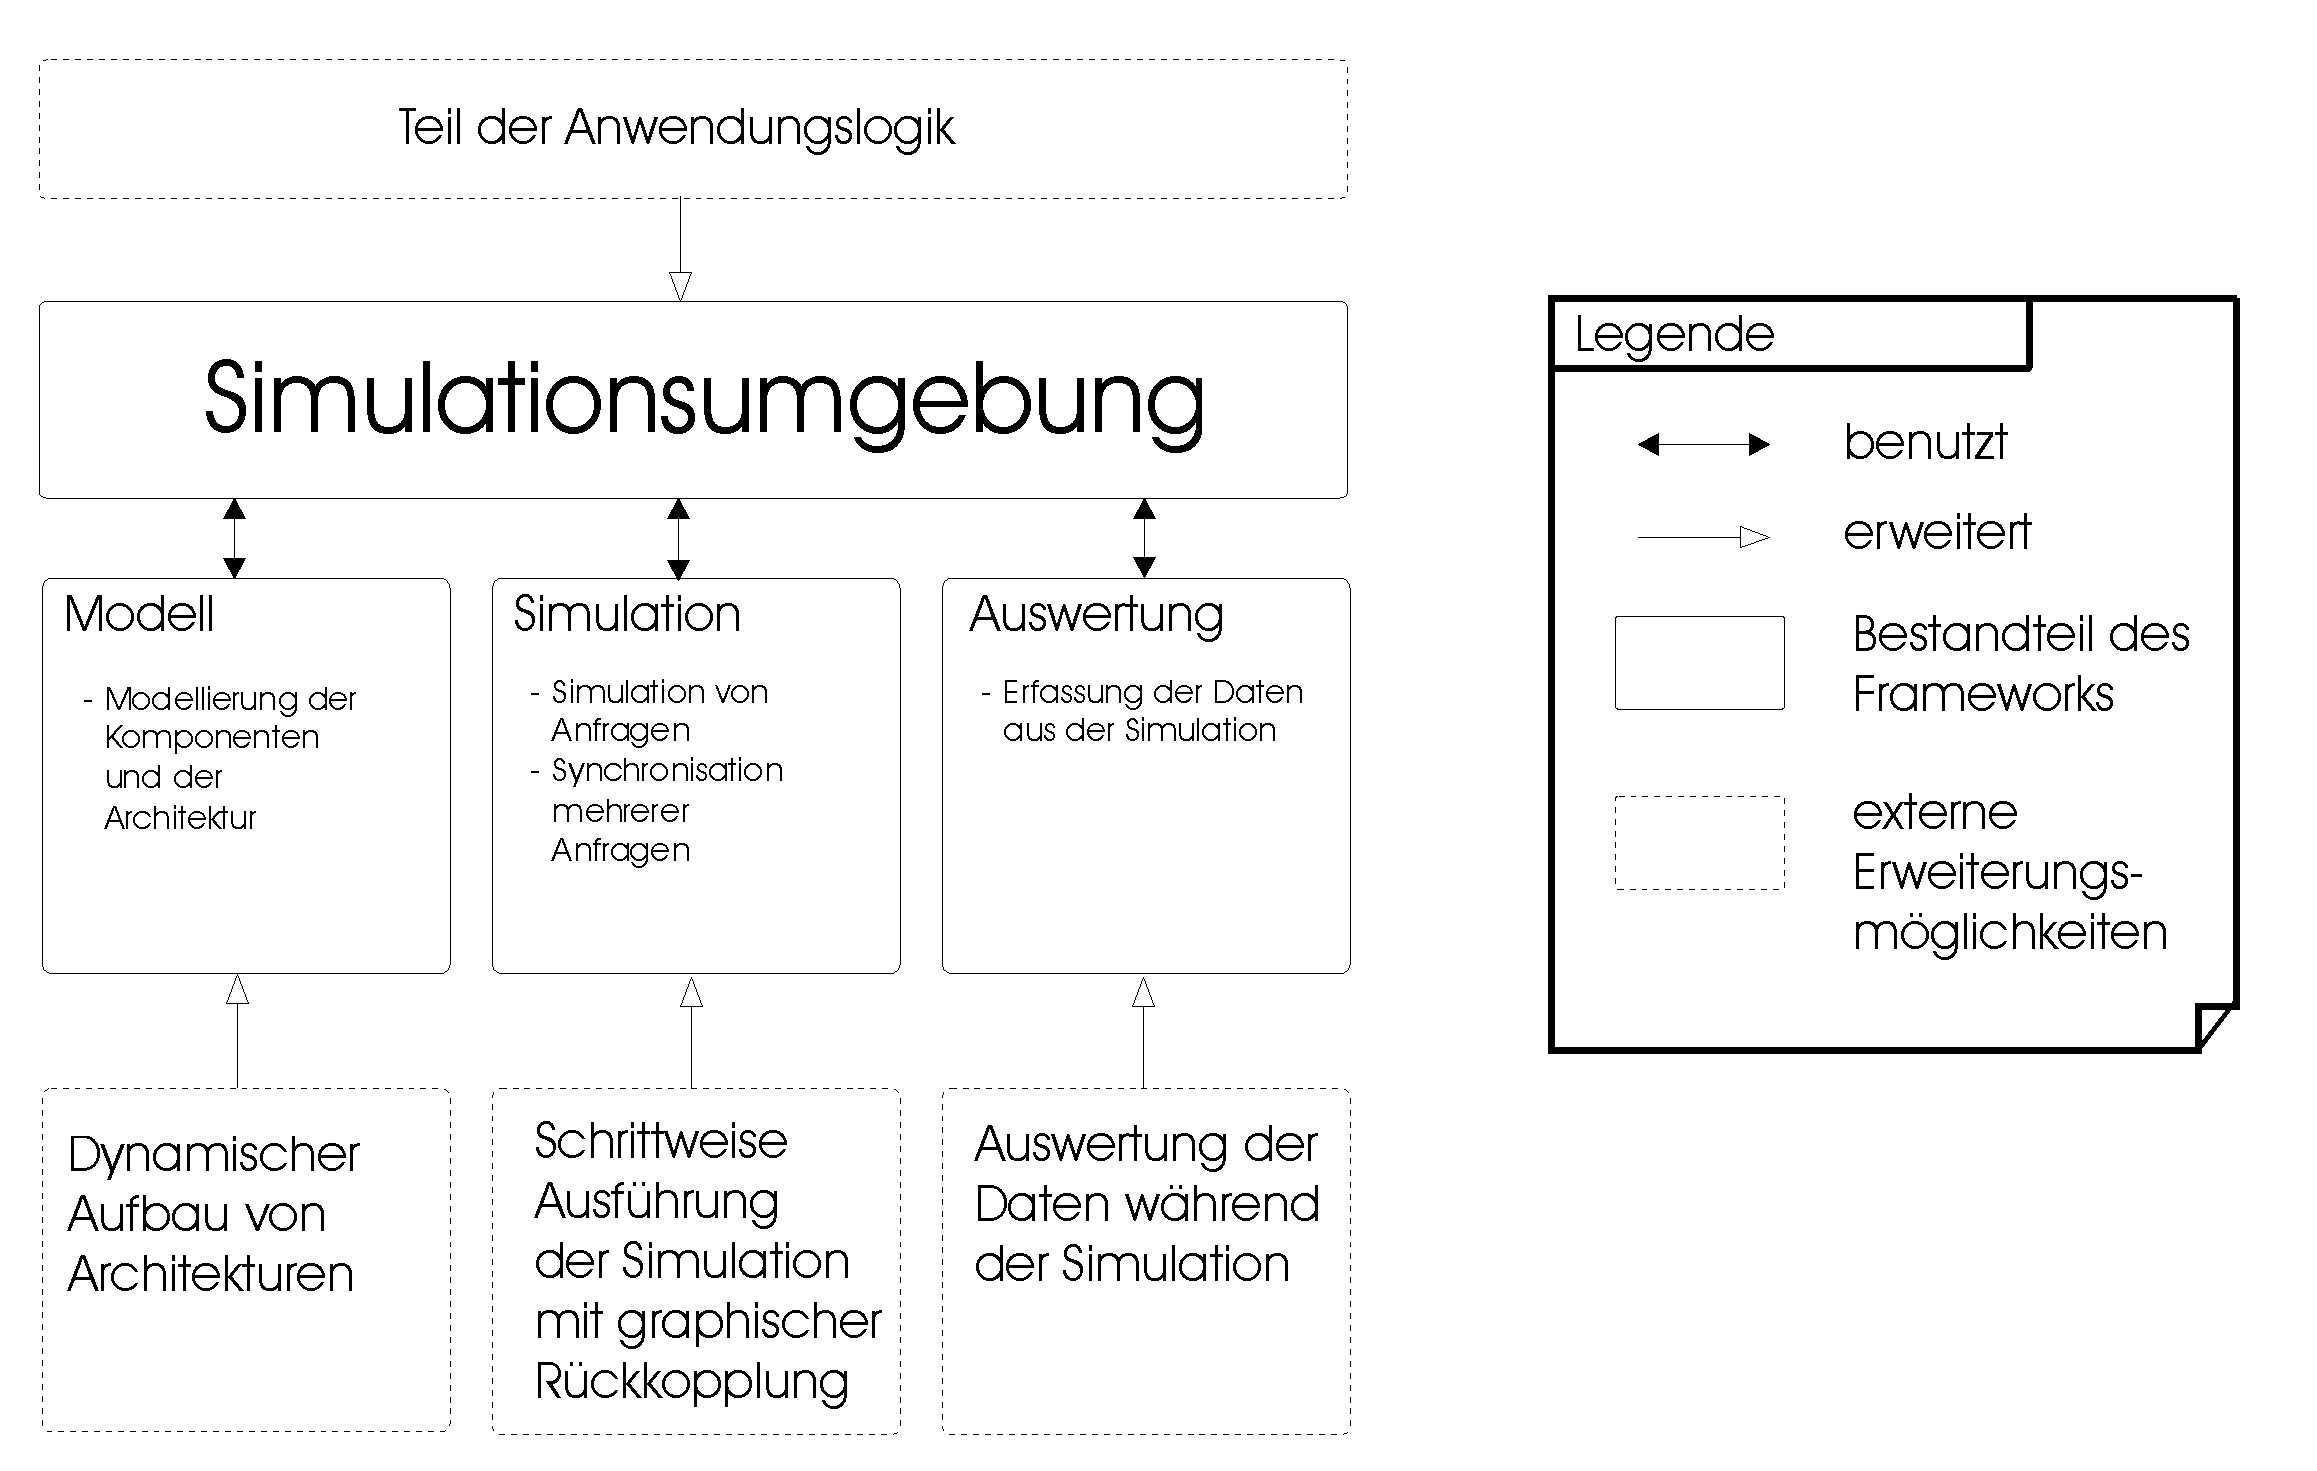
\includegraphics[width=13.5cm]{../res/architektur.png}
\caption{Architektur des Frameworks mit Erweiterungsm�glichkeiten}
\label{pic:architecture}
\end{center}
\end{figure}

Im Folgenden werden jetzt die drei oben erw�hnten Bestandteile und die Verbindungsebene einzeln genauer beleuchtet und die zu ihrer Umsetzung ben�tigten Komponenten identifiziert.

\subsubsection {Bestandteile der Simulationsumgebung}
\label{sec:entwurf:grob:umgebung}
Wie oben erl�utert, besteht die Hauptaufgabe der Simulationsumgebung in der Koordinierung der Kommunikation der anderen Bestandteile des Frameworks. Hierzu m�ssen in diesem Teil die verwendeten Instanzen der anderen Bestandteile gehalten und bei der Initialisierung miteinander verkn�pft werden. Weiterhin sollen Teilkomponenten des Frameworks m�glichst austauschbar sein, ohne die Simulationsumgebung selbst oder andere gr��ere Teile ver�ndern zu m�ssen. Solche �nderungen sollen lediglich beim Erweitern um neue Funktionalit�ten n�tig sein. Das bedeutet, dass alle Bestandteile des Frameworks �ber die Simulationsumgebung konfigurierbar sein m�ssen.

\subsubsection{Bestandteile des Modells}
\label{sec:entwurf:grob:modell}
Wie in Kapitel  \ref{sec:modell:grundlagen} beschrieben, besteht das Modell aus der Modellierung der Komponenten, deren Diensten und den Verbindungen zwischen ihnen. Im Framework soll als Basisfunktionalit�t lediglich der Aufbau jedoch nicht die Ver�nderung der Architektur zur Verf�gung gestellt werden. Es m�ssen also zur Architektur Komponenten hinzugef�gt, diese miteinander verbunden und mit Diensten und Schnittstellen gef�llt werden. Weiterhin m�ssen die Zeitverbraucher im Modell geeignet modelliert und mit dem Modell dem Simulationsteil zur Verf�gung gestellt werden. Zus�tzlich soll der Aufbau der Architektur �berwachbar sein, damit z.B. eine angeschlossene visualisierende Komponente den Aufbau der Architektur nachvollziehen kann. Eine weitere wichtige Anforderung an das Modell ist die Erweiterbarkeit um Zeitverbraucher mit unterschiedlichstem Verhalten. Somit muss die Modellierung eines Zeitverbrauchers vollkommen unabh�ngig von der oben beschriebenen aufbauenden Komponente sein. Damit die f�r ein Modell zu verwendenen Zeitverbraucher ohne gro�artige �nderungen im Framework hinzugef�gt werden k�nnen, muss die aufbauende Komponente, wie im vorherigen Abschnitt beschrieben, �ber die Simulationsumgebnung mit dem angebotenen Set von Zeitverbrauchern konfiguriert werden.

\subsubsection{Bestandteile der Simulation}
\label{sec:entwurf:grob:sim}
Das in Kapitel \ref{sec:modell:simulation} aufgestellte Modell ben�tigt zu seiner Umsetzung zwei Komponenten, die eigentlichen {\em Simulationsthreads} und einen {\em Scheduler}.\\
Die Threads halten alle Daten der Anfrage, die sie simulieren. Hierzu geh�rt der momentane Aufenthaltsort innerhalb der Komponentenarchitektur, der Weg dorthin  und die Zeit, bis der Thread zum n�chsten zeitverbrauchenden Element wechseln kann. Weiterhin ben�tigen sie Informationen dar�ber, welche Daten sie zu sammeln haben. Hier bieten sich drei M�glichkeiten:
\begin{enumerate}

\item Der Thread sammelt �berhaupt keine Daten. Diese Threads eignen sich in Verbindung mit anderen Threads, um Belastungen zu simulieren, die dann andere Threads in ihrer Ausf�hrung beinflussen.

\item Der Thread protokolliert alle Elemente der Komponentenarchitektur, die eine Markierung tragen.

\item Der Thread protokolliert alle Elemente auf seinem Weg.

\end{enumerate}

Der Scheduler dient der Verwaltung der Threads. Er sorgt f�r die Erstellung neuer Threads, die Berechnung der Gr��e des n�chstm�glichen Simulationsschrittes und die Entfernung von beendeten Threads.\\
Neben den einmalig erzeugten, soll das Framework auch regelm��ig wiederkehrende Anfragen modellieren k�nnen. Hierf�r werden Threads ben�tigt, die periodisch nach einer bestimmten Zeit einen neuen Thread an der Stelle starten, an der sie selbst gestartet wurden. Theoretisch kann eine Simulation unter Verwendung solcher Threads unendlich lange fortgesetzt werden, da immer wieder neue Threads erzeugt werden. Um solche Simulationen jedoch gezielt laufen lassen zu k�nnen, muss eine maximale Zeit angegeben werden, nach der die Simulation beendet wird. Hierf�r wird eine weitere Komponente ben�tigt, welche durch Aufaddierung der Zeitschritte eine absolute Simulationszeit generiert. Diese im Folgenden als {\em Uhr} oder {\em Clock} bezeichnete Komponente dient au�erdem der zeitlichen Zuordnung der von den Threads erzeugten Simulationsdaten.

\subsubsection{Bestandteile der Datenerfassung}
\label{sec:entwurf:grob:erfassung}
Zur Erfassung von Daten gen�gen an dieser Stelle ereignisgetriebene Komponenten, die �ber die Simulationsumgebung im Simulationsteil des Frameworks registriert werden. Von dort aus werden verschiedene Nachrichten an die Komponenten versendet. 

\subsection{Erl�uterungen zum Feinentwurf}
\label{sec:entwurf:fein}

An dieser Stelle der Entwurfsbeschreibung wird nun auf einige f�r das bessere Verst�ndnis relevante Entwurfsentscheidungen in den vier Bestandteilen des Frameworks eingegangen.

\subsubsection{Palladio Bibliotheken als Basis des Modells}
\label{sec:entwurf:fein:palladio}
Als Basis des Modells dient die Palladio Bibliothek \quellcode{Palladio.ComponentModel}. Diese und einige von ihr ben�tigte Bibliotheken (Palladio.FiniteStateMachine, etc.) stellen die n�tige Infrastruktur zum Aufbau des in Kapitel \ref{sec:modell} erl�uterten Modells zur Verf�gung. Das Framework erweitert lediglich einige Bestandteile der Bibliothek um zeitliche Aspekte. Eine technische Beschreibung der Bibliothek findet man in \cite{lit:cmmodel}.

\subsubsection{Instanziierung und Kommunikation unter Verwendung der Simulationsumgebung}
\label{sec:entwurf:fein:simum}

Den Einstiegspunkt in das Framework bildet die Simulationsumgebung, da diese, wie in der Beschreibung der Architektur erl�utert, f�r die Kommunikation und Instanziierung der drei anderen Bestandteile des Frameworks zust�ndig ist.

\begin{figure}[ht]
\begin{center}
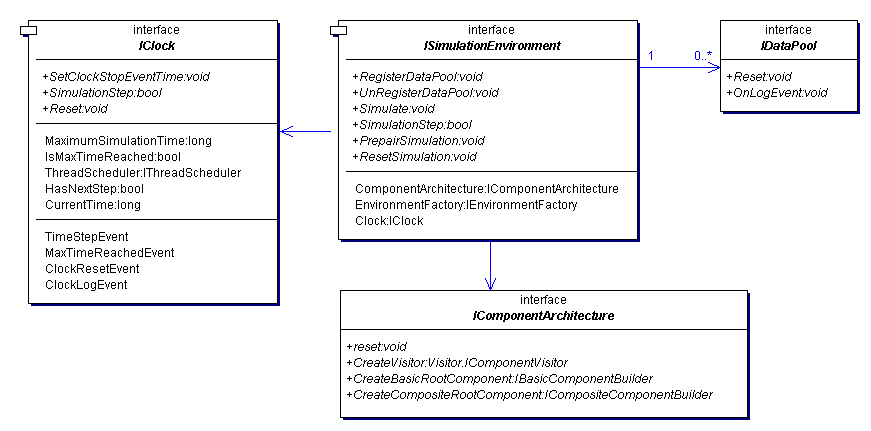
\includegraphics[width=12cm]{../res/simenv.png}
\caption{Zusammenhang Simulationsumgebung und Hauptinterfaces}
\label{pic:simenv}
\end{center}
\end{figure}

Sie wird durch das Interface \quellcode{ISimulationEnvironment} repr�sentiert. Die drei weiteren Teile des Frameworks werden �ber deren Hauptinterface mit der Simulationsumgebung verbunden. Der Zusammenhang zwischen den Interfaces ist im Klassendiagramm in Abbildung \ref{pic:simenv} dargestellt. Hierbei wird der Modellteil durch das Interface \quellcode{IComponentArchitecture} und der Simulationsteil durch das Interface \quellcode{IClock} definiert. Die Komponenten, welche der Datenerfassung dienen, implementieren das Interface \quellcode{IDataPool}. Wird eine neue Simulationsumgebung erstellt, so hat diese f�r die Instanziierung der \mbox{\quellcode{IClock}} und \quellcode{IComponentArchitecture} implementierenden Klassen zu sorgen und diese �ber die in \quellcode{ISimulationEnvironment} definierten Eigenschaften zur�ckzugeben. Die Datenerfassungskomponenten m�ssen nicht zwingend durch die Simulationsumgebung erstellt werden, da sie keinerlei Bedarfsdienste der anderen Klassen des Frameworks enthalten. Sie werden ausschlie�lich unter Verwendung von Events angesprochen und k�nnen in der Simulationsumgebung in beliebiger Anzahl registriert werden. Die Eigenschaften \quellcode{Clock} und \quellcode{ComponentArchitecture} dienen der Kommunikation. Die Vorimplementierungen von \quellcode{IClock} und \quellcode{IComponentArchitecture} beispielsweise werden mit der Instanz der Simulationsumgebung erstellt und k�nnen so �ber die Eigenschaften auf die tats�chliche Instanz der anderen Klasse zugreifen. Ziel der Entwurfsentscheidung ist die Entkoppelung der drei Hauptbestandteile des Frameworks, die sich hiermit einzeln unabh�ngig voneinander ersetzen lassen.
\par
Um kleinere �nderungen oder Anpassungen des Frameworks ohne Neuimplementierung des jeweiligen Hauptinterfaces und damit auch der eigentlichen Simulationsumgebung vornehmen zu k�nnen, m�ssen die Vorimplementierungen konfigurierbar sein. Im Framework wird hierf�r eine Fabrik eingesetzt, deren Instanz ebenfalls in der Simulationsumgebung gehalten wird. Die Eigenschaft \quellcode{EnvironmentFactory} gibt diese zur�ck. Abschnitt \ref{sec:entwurf:fein:konf} geht auf den Aufbau und die Benutzung der Fabrik genauer ein.
\par
Die Vorimplementierung der Simulationsumgebung befindet sich in der Klasse \quellcode{DefaultSimulationEnvironment} und ist direkt instanziierbar. Benutzt man deren parameterlosen Konstruktor, wird die Fabrik des Frameworks zur Konfiguration benutzt. Einem weiteren Konstruktor kann eine eigene Implementierung der Fabrik �bergeben werden. Zwischen der instanziierbaren Klasse der Simulationsumgebung und deren Interface befindet sich die abstrakte Klasse \quellcode{AbstractSimulationEnvironment}, welche einen Teil der Implementierung bereits enth�lt und einem Nutzer des Frameworks die Erstellung einer neuen Simulationsumgebung erleichtern kann.

\subsubsection{Modellierung der Zeitverbraucher}
\label{sec:entwurf:fein:timeconsumer}

Zur Modellierung aller m�glichen Zeitverbraucher des Frameworks dient das Interface \quellcode{ITimeConsumer}, das von allen Bestandteilen des Modells implementiert werden muss, die im Kontrollfluss Zeit verbrauchen sollen. Endeckt der Simulationsthread in seinem Kontrollfluss ein Objekt, welches das Interface implementiert, so wird dessen Zeit in die Simulation einflie�en.\\
\quellcode{ITimeConsumer} enth�lt die folgenden drei Methoden:
\begin{itemize}
\listitem {ThreadEntered()}
Diese Methode wird vom Simulationsthread aufgerufen, sobald es in den Zeitverbraucher eintreten m�chte, um zu erfahren, welche Zeit verbraucht werden muss.

\listitem {ThreadExited()}
Nach Ablauf der Wartezeit wird der Simulationsthread den Zeitverbraucher wieder verlassen. Um dem Zeitverbraucher das Verlassen mitzuteilen, wird \quellcode{ThreadExited()} aufgerufen. W�hrend im statischen Fall der Aufruf ignoriert werden kann, m�ssen dynamische Zeitverbraucher hier ihre Wartezeit �ndern, wenn diese von den im Moment im Zeitverbraucher befindlichen Threads abh�ngt.

\listitem {Reset()}
\quellcode{Reset()} wird von der Simulationsumgebung aufgerufen, um die gesamte Simulation zur�ckzusetzen. Das bedeutet f�r dynamische Zeitverbraucher, dass sie an dieser Stelle ihre Startkonfiguration wieder herzustellen haben.

\end{itemize}

Die Eigenschaft \quellcode{LoggingType} legt fest, ob der Zeitverbraucher einen Messpunkt in der Simulation darstellt. Messpunkte k�nnen beim Eintritt in den Zeitverbraucher, beim Austritt oder in beiden F�llen ein Event im Thread ausl�sen, welches dann zwecks Datenerfassung zu den Auswertungskomponenten weitergeleitet wird. Welche Threads an welcher Stelle Daten erfassen, wird in Abschnitt \ref{sec:entwurf:fein:sim} detailliert erl�utert. Abbildung \ref{pic:timeconsumer} zeigt das Interface und seine Methoden.
 
\begin{figure}[ht]
\begin{center}
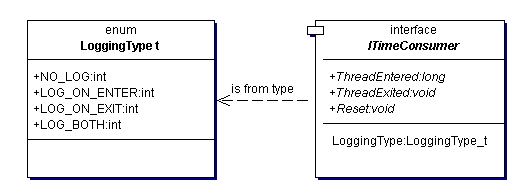
\includegraphics[width=10cm]{../res/timeconsumer.png}
\caption{Interface der Zeitverbraucher}
\label{pic:timeconsumer}
\end{center}
\end{figure}

In Kapitel \ref{sec:modell} wurden die Verbindungen zwischen zwei Komponenten (Bindings) und die Zust�nde der Dienstbedarfsautomaten als potentielle dynamische Zeitverbraucher identifiziert. Sie werden im Framework durch die Interfaces \quellcode{ISimulationBinding} und \quellcode{ISimulationState} definiert.
\quellcode{ISimulationBinding} und \quellcode{ISimulationState} sind Erweiterungen der Interfaces \quellcode{IBinding} und \quellcode{IState} aus Palladio.ComponentModel (siehe Abschnitt \ref{sec:entwurf:fein:palladio}) um Zeitverbraucherinformationen also um das Interface \quellcode {ITimeConsumer}.
W�hrend die Bindings mit dieser Erweiterung vollst�ndig beschrieben sind, erhalten die Zust�nde zus�tzlich die Eigenschaft \quellcode{ControlFlowStrategy} des Typs \quellcode{IControlFlowStrategy}. Die �ber diese Eigenschaft 
referenzierte Instanz einer Klasse dient der Aufl�sung des Nichtdeterminismus, welcher an einem Zustand mit mehreren ausgehenden Transitionen oder an einem Endzustand mit einer und mehr ausgehenden Transitionen entsteht. Das Framework bietet hier eine vorimplementierte Zufallsstrategie (\quellcode{DefaultRandomStrategy}) an, welche die n�chste zu nehmende Transition per Zufall ausw�hlt.
\par
Das Framework enth�lt zu beiden Interfaces zum Teil vorimplementierte abstrakte Klassen, die im wesentlichen die unver�nderte Funktionalit�t der Bindings und States an die jeweilige Implementierung der Bibliothek delegieren. Sie dienen der vereinfachten Erweiterbarkeit und k�nnen zur Erstellung von Bindings und States mit unterschiedlichstem Verhalten einfach �berschrieben werden. Zus�tzlich bietet das Framework f�r die beiden Zeitverbraucher zwei vorimplementierte Klassen, welche den statischen Fall abdecken. Sie modellieren jeweils Zeitverbraucher mit einer festen Zeit. Die Benutzung der Vorimplementierungen und die Erweiterung um neue Arten von Zeitverbrauchern wird im folgenden Abschnitt erl�utert.

\subsubsection{Erweiterung des Frameworks um neue Zeitverbraucher}
\label{sec:entwurf:fein:neuezv}

Eine der Hauptanforderungen an das Framework stellt die Erweiterbarkeit um Zeitverbraucher mit unterschiedlichstem dynamischen Verhalten dar. Hierzu k�nnen die im vorherigen Abschnitt erl�uterten abstrakten Klassen erweitert oder die Interface komplett neu implementiert werden. Voraussetzung f�r die Implementierung von verschiedensten Verhaltensweisen ist eine beliebige Art und Anzahl von Parametern, die den Zeitverbrauchern bei der Erstellung zur Verf�gung stehen m�ssen. W�hrend beispielsweise ein statischer Zeitverbraucher mit einer festen Zeit konfiguriert werden kann, ben�tigt ein die Auslastung modellierender Zeitverbraucher zus�tzlich einen Faktor, der die Erh�hung der Zeit pro Thread beschreibt. Um die Funktionalit�t des Frame\-works zum Aufbau des Modells jedoch unabh�ngig von den Parametern gestalten zu k�nnen, m�ssen diese in einer Datenstruktur gekapselt werden, die beliebig erweiterbar ist. Den Zust�nden dient hierf�r das Interface \quellcode {ISimulationStateParams} und den Bindings \quellcode{ISimulationBindingParams}. Sie definieren bereits einige Parameter, die f�r alle Zust�nde bzw. Bindings n�tig sind. Implementierende Klassen k�nnen zus�tzliche Parameter definieren, die dann nur den zu diesen Klassen kompatiblen Zust�nden bzw. Bindings bekannt sind.
\par
Um die neuen Zeitverbraucher im Modell benutzen zu k�nnen, m�ssen sie in das Framework integriert werden. Zur Umsetzung bietet sich das Entwurfsmuster der {\em Factory Method} an. \cite{lit:gof} empfiehlt eine Anwendung dieses Musters, wenn aus einer Reihe von Hilfsklassen eine auszuw�hlen und das Wissen �ber diese Entscheidung an einer Stelle des Frameworks lokalisiert ist. Im Falle dieses Frameworks wird in Abh�ngigkeit von der Klasse der Parameterstruktur entschieden, welcher der Zeitverbraucher zur Modellierung geeignet ist. Ein Nachteil dieses Musters ergibt sich laut \cite{lit:gof} aus der schlechten Erweiterbarkeit. So muss die erzeugende Klasse jedesmal abgeleitet werden, wenn auch nur ein neuer Zeitverbraucher hinzugef�gt werden soll. Als Konsequenz daraus ergibt sich als weiteres Problem die Zusammenf�hrung unabh�ngig parallel entwickelter Reihen von Zeitverbrauchern, da in einem solchen Fall prinzipiell von beiden erzeugenden Klassen abgeleitet werden muss und Mehrfachvererbung in vielen modernen Programmiersprachen vermieden wird.
\par
Da gerade das Hinzuf�gen von neuen Zeitverbrauchern ohne viel zus�tzlichen Programmieraufwand eine elementare Bedingung an das Framework darstellt, kann dieses Muster so nicht direkt angewendet werden. Es wurde statt dessen zur L�sung der eben erl�uterten Probleme ein Konzept entwickelt, welches das Muster der Factory Method zu Laufzeit dynamisch erweiterbar macht. Abbildung \ref{pic:elements} zeigt alle beteiligten Klassen und deren Zusammenhang. 

\begin{figure}[ht]
\begin{center}
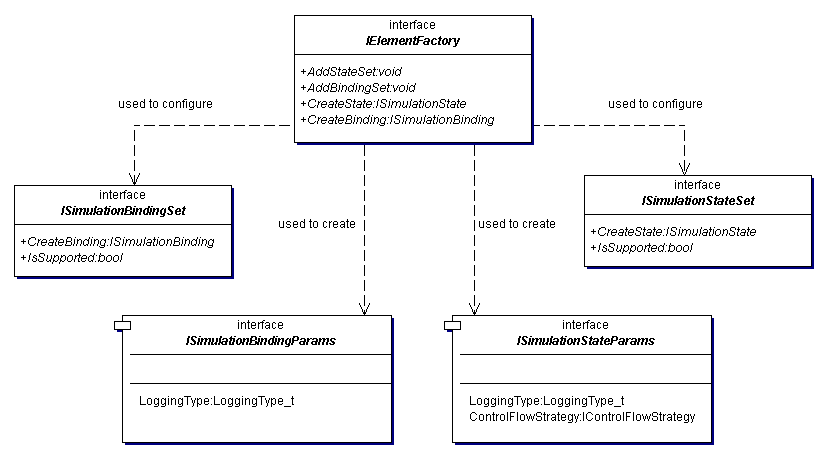
\includegraphics[width=13cm]{../res/elements.png}
\caption{Konfiguration und Erzeugung von Zeitverbrauchern}
\label{pic:elements}
\end{center}
\end{figure}

Das Interface \quellcode{IElementFactory} beinhaltet hierbei die eigentlichen Erzeu\-ger-Methoden \quellcode{CreateState(...)} und \quellcode{CreateBinding(...)}, wie sie aus dem Muster bekannt sind. Diese erzeugen jedoch nicht direkt die Zeitverbraucher sondern iterieren durch eine Liste von State- bzw. Binding-Sets, um eines auszuw�hlen, welches dann den Zeitverbraucher generiert. Diese Sets sind durch die Interfaces \quellcode{ISimulationStateSet} und \quellcode{ISimulationBindingSet} definiert. Ihr Design h�lt sich an das klassische Method Factory Pattern, wie es in \cite{lit:gof} vorgestellt wird. Sie enthalten jeweils eine Create-Methode, welche in Abh�ngigkeit von der �bergebenen Parameterstruktur den Zeitverbraucher erzeugt. Zus�tzlich ist jeweils die Methode \quellcode{IsSupported(...)} definiert, welche zur�ckgibt, ob die angegebene Parameterstruktur vom Set unterst�tzt wird, d.h. ob die Create-Methode unter Verwendung dieser Parameterstruktur einen Zeitverbraucher erzeugen kann.\\
Soll nun ein Zeitverbraucher passend zu einer bestimmten Parameterstruktur erzeugt werden, so iteriert die Create-Methode von \quellcode{IElementFactory} durch alle Sets und �berpr�ft unter Verwendung der Methode \quellcode{isSupported(...)}, ob diese Parameterstruktur unterst�tzt wird. Wurde ein Set gefunden, so wird dieses zum Erzeugen des Zeitverbrauchers benutzt.\\
Zum Hinzuf�gen von neuen Zeitverbrauchern, gen�gt es, ein Set zu schreiben, welches im Stil des Method Factory Pattern die neuen Zeitverbraucher erzeugt. Dieses kann dann dem Framework zur Laufzeit unter Verwendung der Methode \quellcode{AddStateSet(...)} bzw. \quellcode{AddBindingSet(...)} hinzugef�gt werden. Das Interface \quellcode{IElementFactory} ist Bestandteil der Konfiguration des Frameworks und wird in Abschnitt \ref{sec:entwurf:fein:simum} und Abschnitt \ref{sec:entwurf:fein:konf} n�her erl�utert.

\subsubsection{Erstellung des Modells der Architektur}
\label{sec:entwurf:fein:model}

Grunds�tzlich gibt es in der Komponentenarchitektur, welche das Framework unterst�tzt, drei vom Anwender zu f�llende Bestandteile:

\begin{itemize}
\listitem{Basiskomponenten} Bei Basiskomponenten handelt es sich um Komponenten, die ausschlie�lich Dienste enthalten. Das bedeutet, dass beim Aufbau dieser Komponenten Angebots- und Bedarfsschnittstellen und die Dienste selber mit ihrer Signatur hinzugef�gt werden m�ssen.

\listitem{Zusammengesetzte Komponenten} Die zusammengesetzten Komponenten enthalten selber keine Dienste sondern ausschlie�lich andere, m�glicherweise miteinander verbundene Komponenten. Zu ihrem Aufbau m�ssen also M�glichkeiten bestehen, andere Komponenten (Basiskomponenten als auch zusammengesetzte) hinzuzuf�gen und zu verbinden. Weiterhin m�ssen auch hier Angebots- und Bedarfsschnittstellen definierbar sein, damit Dienste der inneren Komponenten nach au�en gef�hrt werden k�nnen.

\listitem{Dienste} Zum Aufbau von Diensten muss die Erstellung der Dienstbedarfsautomaten mit Zust�nden und Transitionen m�glich sein.

\end{itemize}

Der Aufbau der Komponenten und der Dienste wurde im Framework unter Verwendung des Erbauer-Entwurfsmusters (Builder-Pattern) \cite{lit:gof} umgesetzt, um die interne Repr�sentation der Komponenten und Dienste vom Aufbau zu entkoppeln. Es existiert f�r jede der beiden Komponententypen und f�r die Dienste jeweils ein Erbauer, welcher die Methoden zum Aufbau zur Verf�gung stellt. Die Interfaces der einzelnen Erbauer sind der Abbildung \ref{pic:builders} zu entnehmen.

\begin{figure}[ht]
\begin{center}
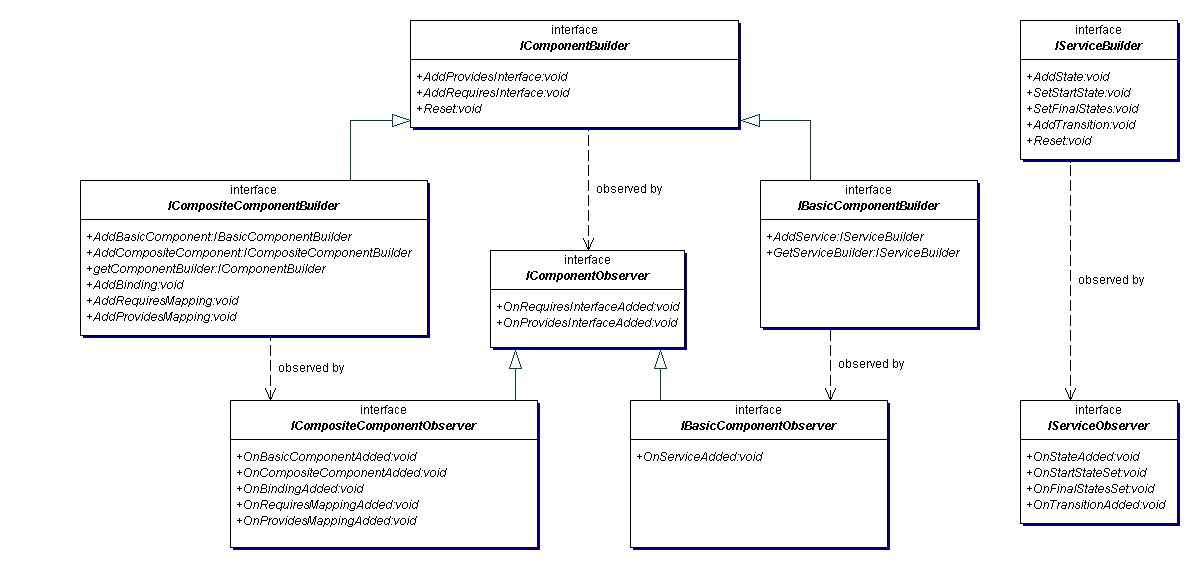
\includegraphics[width=13cm]{../res/builders.png}
\caption{Builder zur Erstellung der Architektur}
\label{pic:builders}
\end{center}
\end{figure}

In der hier umgesetzten Variante des Musters wird der Erbauer selber nicht von au�erhalb des Frameworks instanziiert. Dies geschieht beim Hinzuf�gen einer Komponente. Soll beispielsweise ein Dienst zu einer Basiskomponente hinzugef�gt werden, wird deren Methode \quellcode{AddService()} aufgerufen. Dieser Aufruf f�hrt dazu, dass der internen Repr�sentation der Komponente ein Dienst hinzugef�gt und ein Erbauer erstellt wird, welcher f�r das F�llen des Dienstes zust�ndig ist. Dieser wird nach Verlassen der Methode zur�ckgegeben. Da sich hierbei der Aufbau der Architektur von au�en nach innen gestaltet, bleibt die Frage nach dem Anfang offen. Den Anfang einer Komponentenarchitektur bildet entweder eine zusammengesetzte Komponente oder eine Basiskomponente. Zum Erstellen dieser Komponente enth�lt das Hauptinterface des Modellteils (\quellcode{IComponentArchitecture}) die beiden Methoden \quellcode{CreateBasicRootComponent(...)} und \quellcode{CreateCompositeRootComponent(...)}, welche den entsprechenden Erbauer zu der Komponente zur�ckgeben.
\par

Um den Aufbau der Architektur �berwachbar zu gestalten, kann beim Hinzuf�gen einer Komponente oder eines Dienstes ein �berwacher registriert werden, der bei �nderungen an der Komponente oder dem Dienst benachrichtigt wird. Es handelt sich bei diesem Konstrukt um die Umsetzung des Beobachter-Musters (Observer-Pattern) aus \cite{lit:gof}. Der Zusammenhang zwischen den Erbauern und den �berwachern ist in Abbildung \ref{pic:builders} dargestellt.

\subsubsection{Simulationsthreads, Scheduler und Clock}
\label{sec:entwurf:fein:sim}

Der Simulationsteil besteht aus den in Kapitel \ref{sec:entwurf:grob:sim} identifizierten Teilkomponenten {\em Clock} und {\em Scheduler} und den {\em Simulationsthreads}. Sie werden im Framework durch die Interfaces \quellcode{IClock}, \quellcode{IThreadScheduler} und \quellcode{ISimulationThread} repr�sentiert, wobei \quellcode{IClock} das Hauptinterface des Simulationsteils darstellt und somit direkt �ber die Simulationsumgebung zugreifbar ist (siehe Abschnitt \ref{sec:entwurf:fein:simum}). Simulationsthreads des Typs \quellcode{IPeriodicSimulationThread} bilden eine Erweiterung der Simulationsthreads. Sie veranlassen den Scheduler nach Ablauf einer Periodendauer dazu, einen neuen periodischen Thread an der Stelle zu erzeugen, an der auch sie selber gestartet wurden. Der Zusammenhang dieser Interfaces wird in Abbildung \ref{pic:simulation} verdeutlicht.

\begin{figure}[ht]
\begin{center}
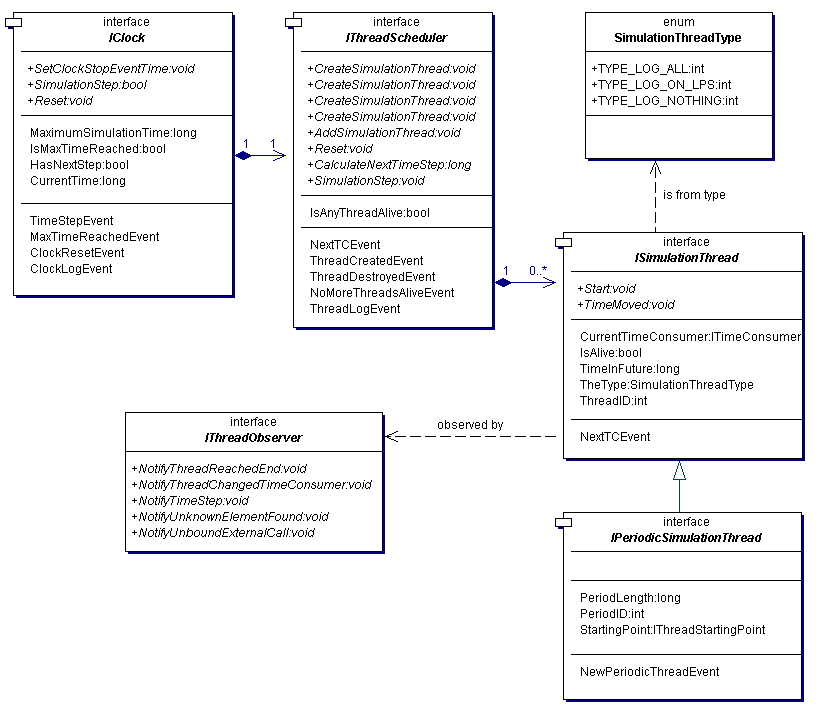
\includegraphics[width=13cm]{../res/simulation.png}
\caption{Klassen und Interfaces des Simulationsteils}
\label{pic:simulation}
\end{center}
\end{figure}

Die Uhr (\quellcode{IClock}) dient der Bildung der Simulationszeit. Damit �berwacht sie die Einhaltung der maximalen Simulationszeit und kann den Datenerfassungskomponenten das Referenzsignal zu den erfassten Daten geben. Neben der Simulationszeit bietet die Uhr mehrere Events, die bei bestimmten Zustands�nderungen der Uhr ausgel�st werden. So wird beispielsweise nach jedem Zeitschritt ein \quellcode{TimeStepEvent} ausgel�st, welches auswertenden Komponenten die L�nge des eben zur�ckgelegten Zeitschrittes �bergibt. 
Die L�nge eines Zeitschrittes berechnet sich, wie in Kapitel \ref{sec:modell:simulation} beschrieben, aus den Zeiten zwischen den Zustands�nderungen der Threads. Um unabh�ngig von diesen Zeiten an bestimmten Punkten Zeitschritte zu beenden, bietet die Uhr die Methode \quellcode{SetClockStopEventTime(int time)} zum Setzen dieser Zeitpunkte. Ein Aufruf dieser Methode stellt sicher, dass beim Erreichen der angegebenen Zeit ein \quellcode{TimeStepEvent} ausgel�st wird, auch wenn keiner der Threads nach Ablauf des Zeitschrittes eine Zustands�nderung erf�hrt.
\par
�ber eine Eigenschaft der Uhr l��t sich der Scheduler erreichen, welcher der Verwaltung der Threads dient. Es k�nnen unter Verwendung der Create-Methoden normale und periodische Threads erzeugt werden, wobei die Angabe des Startpunktes und des Threadtyps gen�gt. Die Vergabe der IDs regelt der Scheduler. Zus�tzlich existiert die Methode \quellcode{AddSimulationThread(...)}, mit der dem Scheduler direkt Simulationsthreads hinzugef�gt werden k�nnen. F�r die Erzeugung des Threads ist hierbei die Anwendung verantwortlich. Simulationsthreads werden in beiden F�llen nicht direkt in die Liste der aktiven Threads eingef�gt, weil beim Erzeugen von neuen Threads innerhalb eines Zeitschrittes sonst die Gefahr der Inkonsistenz besteht. So kann es beispielsweise dazu kommen, dass die neuen an das Ende der Liste angeh�ngten Threads gleich in die Bearbeitung des Zeitschrittes einbezogen werden, obwohl sie erst ab dem n�chsten Zeitschritt existieren d�rften. Zur L�sung dieses Problems werden sie erst vorgemerkt und dann nach Abarbeitung des Zeitschrittes �bernommen.
\par
Um alle Threads einzeln �berwachen zu k�nnen, wurde im Framework an dieser Stelle wieder das Entwurfsmuster des Beobachters (Observer) aus \cite{lit:gof} umgesetzt. Eine Implementierung des Beobachterinterfaces \quellcode{IThreadObserver} kann dem Scheduler bei der Erstellung des Threads �bergeben werden. Die Nutzung der in C\# sonst �blichen Events ist an dieser Stelle nicht m�glich, da eine Anwendung, welche Threads unter Verwendung der Create-Methoden erzeugt, keinen direkten Zugriff auf diese Threads erh�lt.
\par
Da nicht immer alle Anfragen an die Komponentenarchitektur detailliert ausgewertet werden m�ssen, wurde die M�glichkeit der Angabe eines Levels zum Loggen eingef�hrt. Hierbei wird beim Erstellen eines Threads einer der drei im folgenden beschriebenden Typen �bergeben.

\begin{itemize}
\listitem{nicht loggen}
Wird ein Thread unter Angabe des Types \quellcode{TYPE\_LOG\_NOTHING} erzeugt, werden keinerlei Daten von diesem Thread erfasst.

\listitem{an Messpunkten loggen}
Der Typ \quellcode{TYPE\_LOG\_ON\_LPS} eines Threads sorgt daf�r, dass nur Informationen an Messpunkten gesammelt werden. Messpunkte werden detailliert in Abschnitt \ref{sec:entwurf:fein:timeconsumer} beschrieben.

\listitem{alles loggen}
Alle Informationen, die ein Thread sammeln kann, werden bei der Angabe des Typs \quellcode{TYPE\_LOG\_ALL} erfasst.

\end{itemize}

\subsubsection{Besuchermuster zum Navigieren im Modell}
\label{sec:entwurf:fein:visitor}

Zur Umsetzung der Threads muss nun ein Weg gefunden werden, durch das Modell entlang des Kontrollflusses des Threads zu navigieren und die Informationen der Zeitverbraucher auszulesen. Es gibt zur L�sung prinzipiell zwei M�glichkeiten, deren Vor- und Nachteile im Folgenden kurz diskutiert werden.

\begin{trivlist}
\listitem{Navigation durch das Modell}
Bei der Navigation durch das Modell sind im einfachsten Fall alle Elemente durch Referenzen zweifach verkettet. Die Navigation entlang des Kontrollflusses ist so einfach durch Referenzierung des jeweils n�chsten Objekts m�glich. Der R�ckweg l��t sich unter Verwendung der zweiten Kette finden. Die Erstellung eines solchen Modells ist bei Listen oder Baumstrukturen leicht umsetzbar. Werden jedoch wie in einer Komponentenarchitektur Elemente unregelm��ig und zum Teil �ber mehrere Hierachieebenen miteinander verbunden, entsteht schnell eine hohe Komplexit�t an n�tigen Verbindungen. Durch eine Variation mit einem Stack l��t sich das Prinzip auch mit einfach verketteten Elementen umsetzen, wodurch die Komplexit�t der Verbindungen reduziert werden kann. Ein weiterer Nachteil beider Varianten dieses Prinzips bildet die Abh�ngigkeit der verketteten Elemente untereinander. So ist es n�tig, dass z.B. der Dienstbedarfsautomat eines Dienstes, welcher im Framework durch einen endlichen Automaten (Finite State Machine) beschrieben wird, Kenntnis �ber seine Komponente besitzt, damit beispielsweise die Verkettung zu einem externen Dienst �berhaupt realisiert werden kann. M�chte man das Modell des endlichen Automaten unabh�ngig vom Komponentenmodell benutzen, so ist dies aufgrund der Abh�ngigkeit nicht sinnvoll m�glich.
	
\listitem{Navigation auf dem Modell}	
Die Navigation auf dem Modell l�st das Problem der Abh�ngigkeit, indem das Wissen �ber die Verbindung zweier Elemente vom Modell selber auf die Navigation verschoben wurde. Hierzu kennt die navigierende Komponente das gesamte Modell und wei� unter anderem anhand von Informationen einzelner Elemente, welches Element des Modells ein m�glicher Nachfolger ist. So enth�lt bei diesem Prinzip beispielsweise die Navigation und nicht der Zustand die Information dar�ber, dass auf einen Zustand eines endlichen Automaten eine Transition folgt. Die Anwendung dieses Prinzips auf die Komponentenarchitektur und die sich daraus ergebenen Vorteile sollen nun anhand eines kurzen Beispiels verdeutlicht werden. Befindet sich die Navigation in einem Startzustand eines Dienstes einer Komponente, so sucht die Navigation aus dem endlichen Automaten die abgehenden Transitionen des Zustandes, um dann eine f�r den weiteren Weg auszuw�hlen. �ber das Eingabesymbol der Transition bestimmt die Navigation, ohne dass der endliche Automat von seiner Komponente wissen muss, die Bedarfsschnittstelle der Komponente, in der der externe Dienst verzeichnet ist. Von dort aus wird dann der weitere Weg des Kontrollflusses gesucht. Ein Nachteil dieses Prinzips zeigt sich, wenn versucht wird, die Navigation an einer Stelle zu unterbrechen und zu einem sp�teren Zeitpunkt von dort aus fortzusetzen. W�hrend bei der Navigation ohne Unterbrechung die hierarchische Anordnung der Elemente bei geschickter Programmierung im Methodenstack gehalten wird, so m�ssen diese Informationen beim Unterbrechen der Navigation gespeichert werden. Es muss der navigierenden Komponente bekannt sein, in welchem Zustand, von welchem Dienst und von welcher Komponente der Kontrollfluss fortgesetzt werden soll.

\end{trivlist}

Aufgrund der besser zu l�senden Probleme der zweiten Methode und der Tatsache, dass das erste Prinzip von der als Basis verwendeten Bibliothek {\em Palladio.ComponentModel} nicht unterst�tzt wird, wurde im Framework die zweite Methode umgesetzt. 
\par

Hierzu bot sich eine Abwandlung des Besucher-Entwurfsmusters(Visitor-Pattern) an. Dieses Entwurfsmuster empfiehlt \cite{lit:gof}, wenn Operationen auf einer Datenstruktur aus Elementen verschiedenster Typen ausgef�hrt werden sollen, ohne diese mit der Datenstruktur zu verschmelzen. Gerade wenn die auszuf�hrenden Operationen stark abh�ngig von anderen Klassen des Systems sind und man diese Abh�ngigkeit nicht auf die Datenstrukturen erweitern m�chte, ist die Umsetzung des Entwurfsmusters sinnvoll. Genau dieser Punkt spricht f�r die Anwendung bei der Navigation durch die Komponentenarchitektur im Framework, da eine Entkoppelung der Architektur von der Simulation sehr w�nschenswert ist.
\par

Nach dem Simualtionsmodell aus Kapitel \ref{sec:modell:simulation} ist die Unterbrechung der Navigation an jedem Zeitverbraucher essentiell. Zur L�sung der oben erw�hnten Probleme bei solchen Unterbrechungen wurden die Teile der Komponentenarchitektur in Hierarchieebenen unterteilt. Unterste Ebene hierbei ist die Basiskomponente mit ihren Diensten, da sie keine weiteren Komponenten beinhalten kann. Die dar�berliegende Ebene bildet eine zusammengesetzte Komponente, welche jedoch auch wieder Teil einer zusammengesetzten Komponente sein kann. Somit bilden die einzelnen Komponenten eine Hierarchie, welche eine Basiskomponente als unterste Ebene besitzt. Das Framework besitzt f�r die beiden unterschiedlichen Ebenentypen je einen Besucher. Durch eine Basiskomponente navigiert der Besucher des Types \quellcode{IBasicComponentVisitor}. F�r die zusammengesetzten Komponenten exisitieren Besucher des Typs \quellcode{ICompositeComponentVisitor}. Beiden gemeinsam ist die Methode \quellcode{NextElement()}, welche zum n�chsten Element im Kontrollfluss wechselt. Das jeweils aktuelle Element gibt die Eigenschaft \quellcode{CurrentElement} zur�ck. Zur Aufl�sung der oben angesprochenen Hierarchie wird f�r jede dort enthaltene Komponente ein passender Besucher erzeugt. Diese Besucher sind dann entlang der Hierarchie untereinander verbunden und delegieren die Methode \quellcode{NextElement()} und die Eigenschaft \quellcode{CurrentElement} an den n�chsten unterhalb liegenden Besucher weiter, bis der letzte erreicht ist. Das in Abbildung \ref{pic:hierarchie1} dargestellte Kontrollflussdiagramm visualisiert dieses Prinzip.

\begin{figure}[ht]
\begin{center}
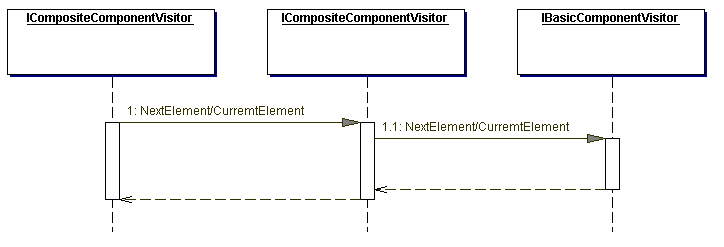
\includegraphics[width=13cm]{../res/hierarchie1.png}
\caption{Kontrollfluss bei drei verschachtelten Komponenten}
\label{pic:hierarchie1}
\end{center}
\end{figure}

Somit ist erreicht, dass die Navigation den genauen Weg zur aktuellen Basiskomponente kennt. Es stellt sich nun die Frage, wof�r dieser Weg so genau bekannt sein muss und warum die zusammengesetzten Komponenten �berhaupt einen Besucher haben m�ssen. Die Antwort ergibt sich aus folgender �berlegung. Neben oben erl�uterter Hierarchie kann sich entlang des Kontrollflusses einer zusammengesetzten Komponente also innerhalb einer der beschriebenen Hierarchieebenen eine zweite Hierarchie bilden. Diese entsteht, wenn der Kontrollfluss durch mehrere hintereinander geschaltete Komponenten verl�uft. Ist die erste Komponente beispielsweise eine Basiskomponente, in der ein externer Dienst einer anderen Basiskomponente aufgerufen wird, so entsteht zwischen diesen beiden Komponeten eine Hierarchie. Im Folgenden wird die erste als �u�ere und die zweite als innere Hierarchie bezeichnet. Abbildung \ref{pic:hierarchie2} verdeutlicht diesen Zusammenhang graphisch.

\begin{figure}[ht]
\begin{center}
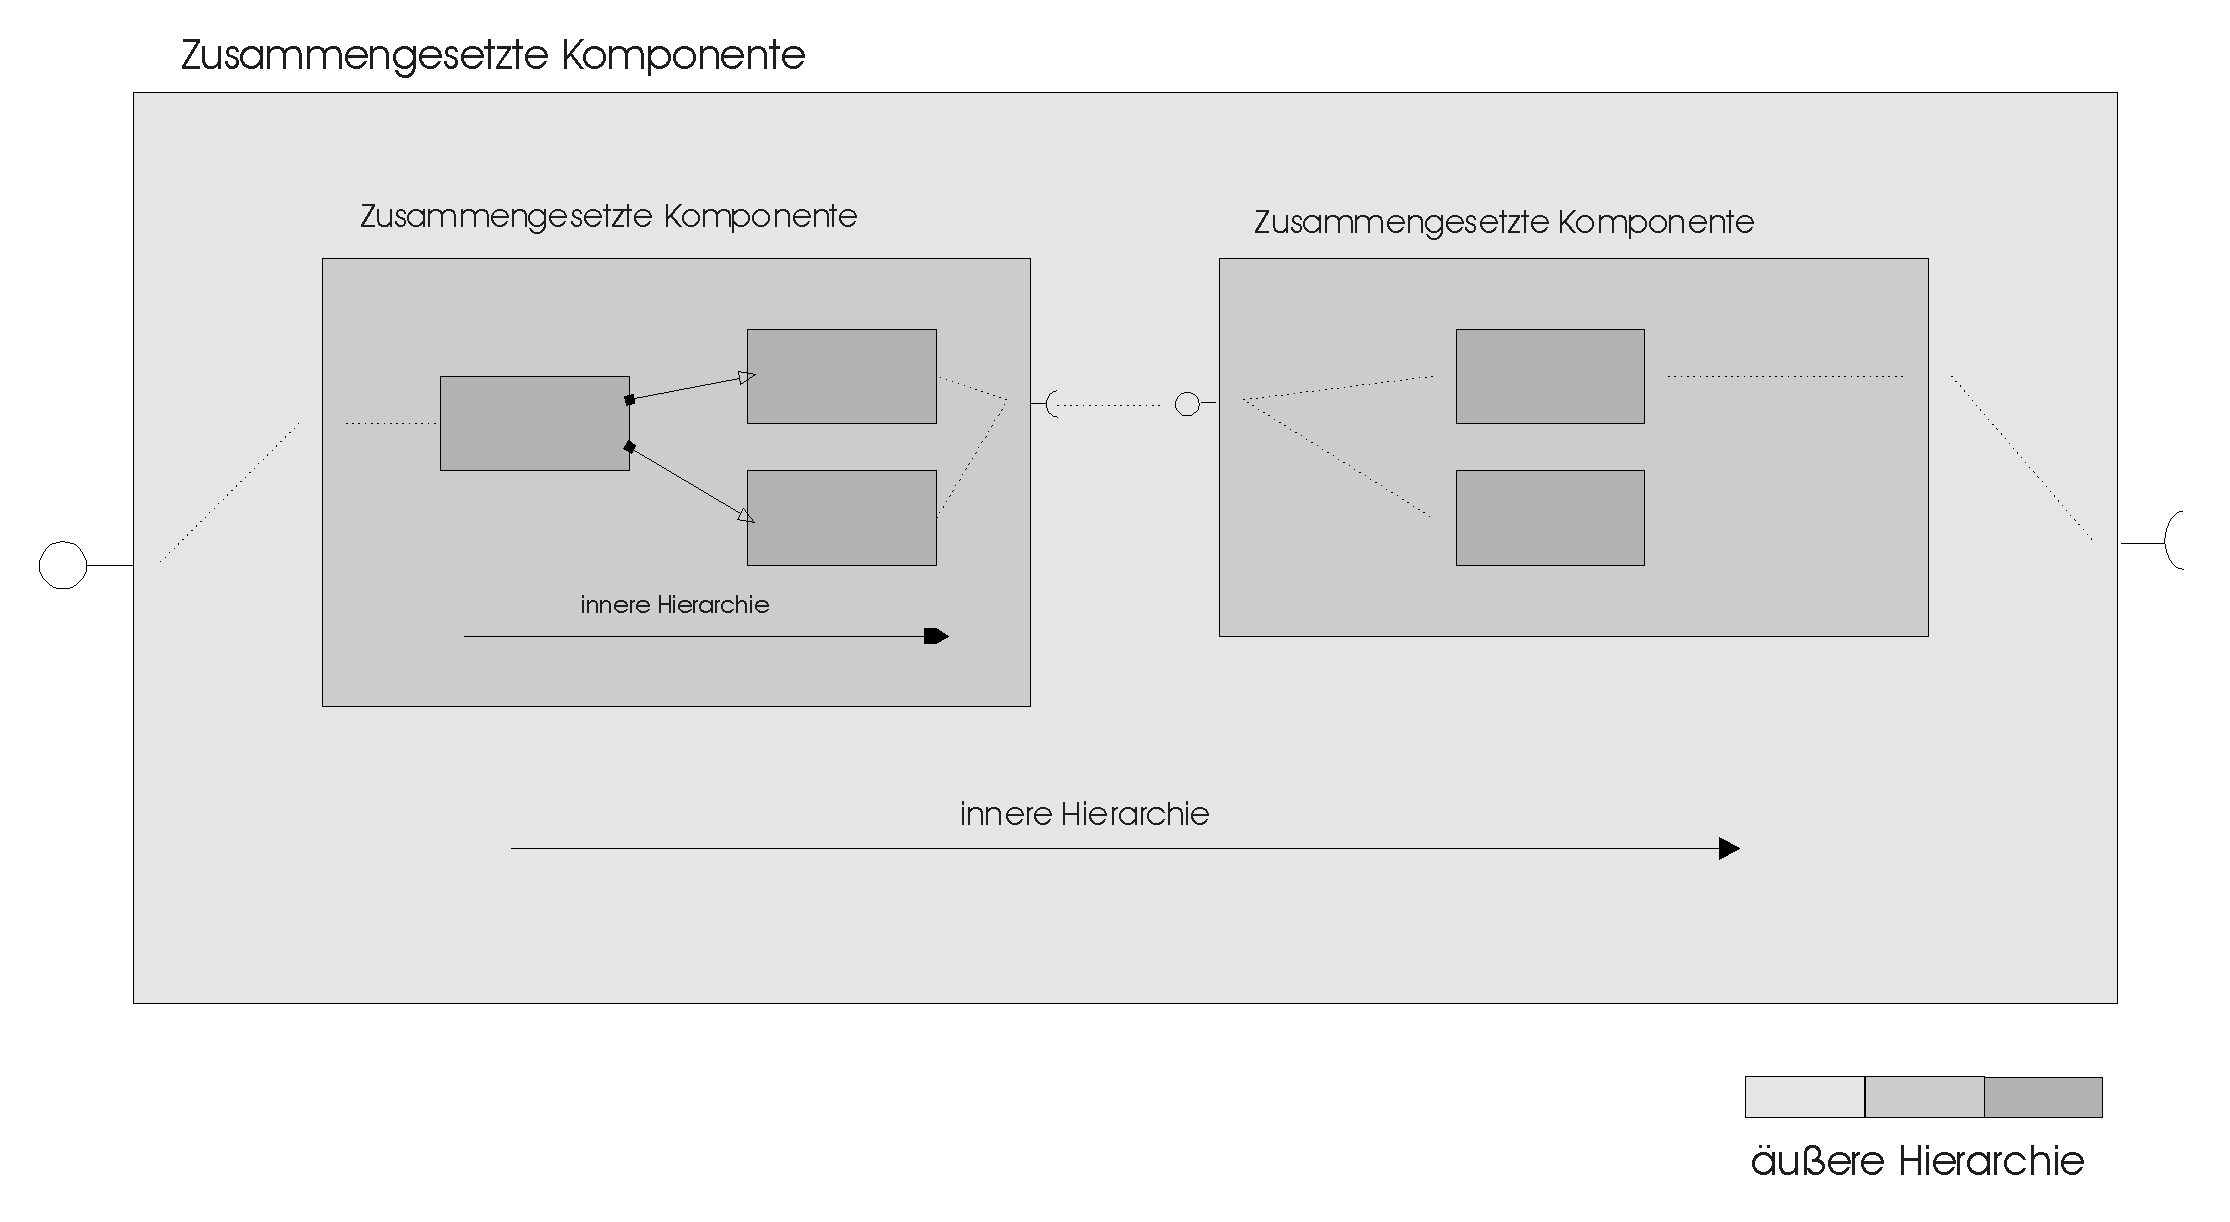
\includegraphics[width=13cm]{../res/hierarchie2.png}
\caption{Unterschied zwischen �u�erer und innerer Hierarchie}
\label{pic:hierarchie2}
\end{center}
\end{figure}

Da aber nun die Basiskomponente keinerlei Kenntnis �ber die Komponente besitzt, welche den externen Dienst implementiert, ist ein Sprung in eine h�here Ebene der �u�eren Hierarchie n�tig, um diese Information zu erfragen. Dort wird bei korrektem Aufbau der Architektur eine Verbindung zu einer anderen Komponente gefunden. Diese kann, wie bei der Identifizierung der Zeitverbraucher in Kapitel \ref{sec:modell:bestandteile} erl�utert, ein dynamischer Zeitverbraucher sein und muss vom Besucher dieser Ebene auch als solcher ausgewertet werden. Hierzu ben�tigen also auch zusammengesetzte Komponenten einen Besucher. Nach dem Verlassen der Verbindung wird eine Komponente betreten, welche in der �u�eren Hierarchie eine Stufe unterhalb der aktuellen liegt. F�r diese wird also ein neuer Besucher eingerichtet und wie oben erw�hnt mit dem Besucher dieser Ebene verkettet. Damit nach der Abarbeitung des externen Dienstes in die aufrufende Komponente zur�ckgesprungen werden kann, muss auch der Weg entlang der inneren Hierarchie gespeichert werden. Hierzu wurde im Framework ein Stack in die Implementierung der Besucher der zusammengesetzten Komponenten integriert, welcher alle Besucher entlang der inneren Hierarchie speichert.

\subsubsection{Datenerfassungsm�glichkeiten}
\label{sec:entwurf:fein:analysis}

Zur Datenerfassung gen�gen, wie in Kapitel \ref{sec:entwurf:grob:erfassung} erw�hnt, passive ereignisgesteuerte Komponenten, welche im Framework durch das Interface \quellcode{IDataPool} repr�sentiert werden. Dieses besitzt die Methode \quellcode{Reset()} zum Zur�cksetzen der Datenerfassung und den Ereignishandler \quellcode{OnLogEvent}. Ein Ereignis f�r die Datenerfasssung zeichnet sich durch die Parameterstruktur des Typs \quellcode{BasicLogEventArgs} aus, welche ausschlie�lich die zu erfassende Nachricht enth�lt. Innerhalb des Frameworks existieren zwei Spezialisierungen dieser Parameterstruktur, \quellcode{ClockLogEventArgs} und \quellcode{ThreadLogEventArgs}. Die erste Erweiterung wird von der Simulationsuhr (\quellcode{IClock}) benutzt und beinhaltet daf�r zus�tzlich eine Referenz auf die Uhr, die L�nge des Zeitschrittes und den Typ des Ereignisses. Die Simulationsthreads senden ihre Informationen unter Verwendung der Parameterstruktur \quellcode{ThreadLogEventArgs} an die Datenerfassung. Hierzu enth�lt diese zus�tzlich die Referenz auf den sendenden Simulationsthread, einen das Ereignis beschreibenden Typ und einen von diesem Typ abh�ngigen Zeitverbraucher. Das in Abbildung \ref{pic:analysis} dargestellte Klassendiagramm zeigt das Interface und die Parameterstrukturen.

\begin{figure}[ht]
\begin{center}
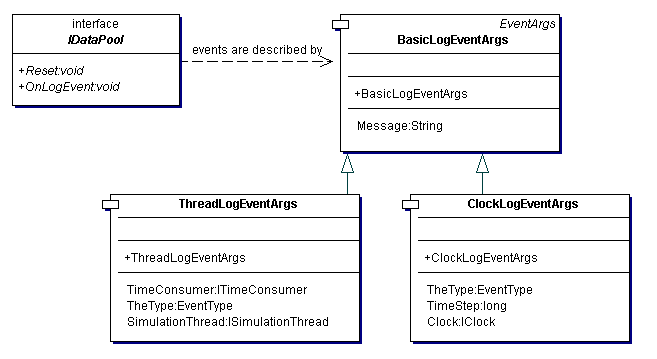
\includegraphics[width=13cm]{../res/analysis.png}
\caption{Datenerfassungskomponente und die Ereignisparameter}
\label{pic:analysis}
\end{center}
\end{figure}

Damit bei Bedarf verschiedene Auswertungskomponenten gleichzeitig Ereignisse verarbeiten k�nnen, besteht die M�glichkeit, mehrere Datenerfassungskomponenten in der Simulationumgebung an- und auch wieder abzumelden. Hierzu dienen die beiden Methoden \quellcode{RegisterDatapool(...)} und \quellcode{UnRegisterDatapool(...)} im Interface der Simulationsumgebung. Diese Architektur bietet prinzipiell sogar die M�glichkeit, ohne Datenerfassungskomponenten zu simulieren. Ein solcher Aufbau macht dann Sinn, wenn die Auswertung der unterschiedlichen Datenquellen nicht sinnvoll an eine Stelle zu bringen ist. Es m�ssen dann eigene Handler geschrieben werden, die bei den Quellen der Ereignisse einzeln registriert werden.

\subsubsection{Konfiguration des Frameworks}
\label{sec:entwurf:fein:konf}

Der letzte Punkt bei der Erl�uterung der Entwurfsentscheidungen widmet sich der Konfiguration des Frameworks. Das Framework l��t sich grunds�tzlich in drei Stufen anpassen. Die erste Stufe der Ver�nderung besteht in der Konfiguration mit neuen Zeitverbrauchern, was zur Laufzeit ohne Ver�nderung von bestehendem Quellcode m�glich ist. Abschnitt \ref{sec:entwurf:fein:neuezv} hat die daf�r entwickelten Konzepte vorgestellt. Die zweite Stufe, deren Umsetzung im Folgenden genauer erl�utert wird, dient der Ersetzung bzw. Erweiterung einzelner Teile der vier gro�en Bestandteile des Frameworks, ohne die Bestandteile selber ver�ndern zu m�ssen. �berschreiten die geplanten Erweiterungen die Grenzen der zweiten Stufe, so m�ssen im Zuge der dritten Stufe Ver�nderungen von einer oder mehrerer der vier gro�en Bestandteile vorgenommen werden. Eine Erweiterung des Modell- oder Simulationsteils zieht hierbei automatisch eine Ver�nderung der Simulationsumgebung nach sich, da diese f�r die Instanziierung der beiden anderen Teile verantwortlich ist. Eine genauere Betrachtung des Zusammenhangs zwischen den Hauptbestandteilen des Frameworks liefert der Abschnitt \ref{sec:entwurf:fein:simum}.
\par
An dieser Stelle werden nun die zur Umsetzung der zweiten Ver�nderungsstufe ben�tigten Konzepte vorgestellt. Der Austausch von Implementierungen an einer Stelle eines Systems ohne Ver�nderung des Systems selber ist eine Musteranwendung des Entwurfsmuster der abstrakten Fabrik (abstract factory). Das diesem Muster zugrundeliegende Prinzip definiert ein Interface gef�llt von �blichweise Fabrikmethoden (factory methods) zur Erzeugung verschiedener Produkte. Zum Austausch dieser Produkte k�nnen dann verschiedene Implementierungen der Fabrik unterschiedliche Instanzen der Produkte erzeugen\cite{lit:gof}.
\par
Das Framework setzt sich aus einer ganzen Reihe solcher potentiell austauschbaren Produkten zusammen, welche verstreut in allen Bestandteilen vorkommen. Beispiele hierf�r sind der Scheduler im Simulationsteil und die einzelnen Zeitverbraucher der Komponentenarchitektur im Modellteil. W�rde man alle diese Produkte mit einer Fabrik erzeugen, so w�rde diese aus einer gro�en Anzahl von Fabrikmethoden bestehen, die z.T. in keinem Zusammenhang stehen. Als Konsequenz einer solchen Entwurfsentscheidung muss bei jedem neuen Produkt die gesamte Fabrik neu erstellt werden. Die Erstellung einer neuen Fabrik l��t sich bei der Anwendung dieses Musters nicht umgehen. Um den Aufwand zu minimieren, wurden nicht alle Produkte in eine Fabrik verpackt. Nur semantisch zusammenh�ngende Produkte sind in einer Fabrik enthalten. Alle so entstandenen Fabriken werden dann in der durch das Interface \quellcode{IEnvironmentFactory} repr�sentierten globalen Fabrik gekapselt. Das Klassendiagramm aus Abbildung \ref{pic:factories} zeigt die Interfaces aller Fabriken und deren Zusammenhang.

\begin{figure}[ht]
\begin{center}
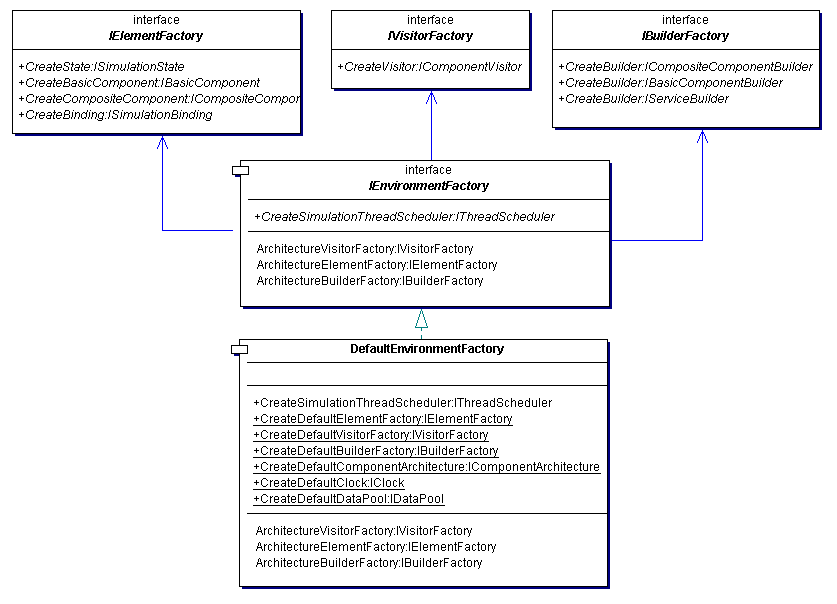
\includegraphics[width=13cm]{../res/factories.png}
\caption{Zusammenhang zwischen den Fabriken zur Konfiguration des Frameworks}
\label{pic:factories}
\end{center}
\end{figure}

Der gro�e Vorteil dieses Entwurfs liegt in der Kapselung logisch zusammenh�ngender Produkte. Liegen beispielsweise eine Reihe solcher Fabriken vor, so k�nnen diese bei der Erstellung einer neuen Anwendung in einer beliebigen Kombination weiterverwendet werden. Die Kapselung in der globalen Fabrik erfordert jedoch f�r jede dieser Kombinationen eine eigene Implementierung dieser Fabrik. W�rde jedoch die Kapselung weggelassen, so m�sste man zur Konfiguration des Frameworks die zu verwendenen Produktfabriken einzeln �bergeben, was aufgrund gegebener Anzahl un�bersichtlich wird.
\par
Alle Basisimplementierungen des Frameworks werden durch Standardfabriken erzeugt, welche in der globalen Fabrik \quellcode{DefaultEnvironmentFactory} gekapselt sind. Diese Klasse wird vom Framework automatisch zur Konfiguration benutzt, wenn keine andere Fabrik �bergeben wurde. Sollen einige der Standardfabriken in einer eigenen globalen Fabrik weiterbenutzt werden, so k�nnen diese unter Verwendung der statischen Methoden aus \quellcode{DefaultEnvironmentFactory} erzeugt und in den entsprechenden Methoden der eigenen globalen Fabrik zur�ckgegeben werden.\\
\par
Nachdem an dieser Stelle ein �berblick �ber den inneren Aufbau des Framework gegeben wurde, folgen im n�chsten Kapitel einige Hinweise zur Anwendung des Frameworks.


\newpage

\section{Anwendung des Frameworks}
\label{sec:anw}
Gem�� der Anforderungsdefinition aus Kapitel \ref{sec:entwurf:anf} besteht das Framework aus einer Reihe vorimplementierter Funktionalit�t, die sich beliebig austauschen und erweitern l��t. Dieses Kapitel beschreibt im ersten Teil die Nutzung dieser Vorimplementierungen. Im zweiten Teil werden einige Erweiterungsm�glichkeiten und die Stellen des Frameworks, an denen sie ansetzten aufgezeigt. Abschlie�end geht dieses Kapitel auf die Grenzen des Frameworks ein.

\subsection{Nutzung der vorimplementierten Funktionalit�t}
\label{sec:anw:vorimpl}

Das Framework gestattet die Erstellung von Simulationen, ohne auch nur eine Klasse des Frameworks �ndern zu m�ssen. Hierzu muss lediglich Quellcode erstellt werden, welcher unter Verwendung des Frameworks das Modell erstellt, Simulationsthreads erstellt und die Simulation startet. Dieser Vorgang wird im folgenden kurz beschrieben.

\subsubsection{Instanzierung des Frameworks}
\label{sec:anw:vorimpl:instanz}

Die Instanzierung des Frameworks gestaltet sich denkbar einfach. Hierzu gen�gt ein einfacher Aufruf des parameterlosen Konstruktors der Vorimplementierung der Simulationsumgebung \quellcode{DefaultSimulationEnvironment}. Eine Konfiguration des Frameworks ist in diesem Fall nicht n�tig. Hierf�r wird vom Framework die globale Fabrik der Vorimplementierungen benutzt.

\subsubsection{Aufbau eines Modells}
\label{sec:anw:vorimpl:modell}

Als n�chstes ben�tigt das Framework das Modell der Architektur, auf dem sp�ter die Simulation ausgef�hrt werden soll. Das Hauptinterface des Modellteils, welches zum Aufbau des Modells ben�tigt wird, wird �ber das Property \quellcode{ComponentArchitecture} der Simulationsumgebung erreicht. Jede Komponentenarchitektur des Frameworks besteht entweder aus einer Basis- oder einer zusammengesetzten Komponente. Diese kann durch eine der beiden Create-Methoden des Modellteils unter Angabe einer ID und eines Beobachter erzeugt werden. Soll die Erstellung der Komponente nicht �berwachbar sein, so kann an Stelle des Beobachters auch \quellcode{null} �bergeben werden. Um die neuen Komponenten f�llen zu k�nnen benutzt man das zur�ckgegebene Interface der Create-Methoden. Handelt es sich um eine Basiskomponente, so stellt das Interface Methoden zum F�llen der Komponente mit Diensten zur Verf�gung.
Wird ein Dienst hinzugef�gt, so erh�lt man ebenfalls ein Interface, welches zum F�llen dieses Dienstes benutzt werden kann. Das Interface zum F�llen der zusammengesetzten Komponenten dagegen enth�lt Methoden zum Hinzuf�gen neuer Komponenten und den Verbindungen dazwischen. Folgener Codeausschnitt verdeutlicht dieses Prinzip anhand der Erzeugung einer Basiskomponente mit einem Dienst.

\footnotesize
\begin{verbatimtab}
...
ISimulationEnvironment env = new DefaultSimulationEnvironment();

//id: the id of the component
IBasicComponentBuilder bcb = env.ComponentArchitecture.
	CreateBasicRootComponent(id,obsBC);

//pIfaceID: id of the provides interface
//sigID: id of the signature for this service 
IServiceBuilder sb = bcb.AddService(pIfaceID,sigID, obsSV);

//parms1,parms2: the parameters of the states
sb.AddState(parms1);
sb.AddState(parms2);

//id1,id2, the ids of the states
sb.SetStartState(id1);
sb.SetFinalStates(new String[]{id2});

//extSigID: id of the signature of the external call
//reqIFaceID: the id of the requires interface
sb.AddTransition(id1, extSigID, reqIFaceID,id2);
...
\end{verbatimtab}
\normalsize

Die Angebots- und Bedarfsschnittstellen k�nnen explizit hinzugef�gt werden. Exisitieren sie beim Hinzuf�gen von beispielsweise einem Dienst noch nicht, so werden sie automatisch passend erzeugt.

\subsubsection{Registrieren von Datenerfassungskomponenten}
\label{sec:anw:vorimpl:daten}

Als n�chstes m�ssen in der Simulationsumgebung Komponenten zur Datenerfassung hinzugef�gt werden. Das Framework bietet hierf�r zwei Exemplare an, welche unter Verwendung der Fabrik \quellcode{DataPoolFactory} erzeugt werden k�nnen. Die erste Komponente schreibt alle erhaltenen Daten auf die Console. Sie l��t sich mit der Methode \quellcode{CreateConsoleWriterDataPool(...)} erzeugen. Der zweiten Komponente kann ein \quellcode{TextWriter} Objekt �bergeben werden, in das die Daten geschrieben werden. Diese l��t sich unter Verwendung der Methode \quellcode{CreateTextWriterDataPool(...)} erstellen. Wurde eine Instanz einer Datenerfassungskomponente erstellt, so kann sie in Simulationsumgebung registriert werden. Die folgenden Codezeilen erzeugen die erste der beiden Komponenten und registriert sie in der Umgebung.

\footnotesize
\begin{verbatimtab}
...
//env: instance of ISimulationEnvironment
IDataPool dp = DataPoolFactory}.CreateConsoleWriterDataPool(env);
env.RegisterDataPool(db);
...
\end{verbatimtab}
\normalsize

\subsubsection{Erstellung von Simulationsthreads und Starten der Simulation}
\label{sec:anw:vorimpl:sim}

Bevor nun die Simulation gestartet werden kann, m�ssen Simulationsthreads an einer beliebigen Stelle der Architektur erzeugt werden. Hierf�r bietet der Scheduler des Simulationsteils verschiedene Methoden an, mit denen normale und periodische Threads mit oder ohne Beobachter erzeugt werden k�nnen. Die Stelle, an der der Thread gestartet werden soll, wird hierbei durch eine Instanz des Interfaces \quellcode{IThreadStartingPoint} definiert, die die Komponente, die Angebotsschnittstelle und die Signatur des Dienstes zur�ckgibt. Folgender Quelltext erzeugt ein normales Simulationsthread in der Komponente 'Comp' an der Signatur 'd1' der Angebotsschnittstelle 'P1' und f�hrt dann unter Verwendung der Methode \quellcode{Simulate()} der Simulationsumgebung die Simulation aus.

\footnotesize
\begin{verbatimtab}
...
//env: instance of ISimulationEnvironment
IThreadStartingPoint sp = new 
		DefaultThreadStartingPoint(ID("Comp"),ID("P1"),ID("d1"));

env.Clock.ThreadScheduler.CreateSimulationThread(sp,
	SimulationThreadType.TYPE_LOG_ALL);
	
env.Simulate();
...
\end{verbatimtab}
\normalsize

\subsection{Erweiterungsm�glichkeiten}
\label{sec:anw:erweit}

Die Erweiterung des Frameworks unterteilt sich, wie in Kapitel \ref{sec:entwurf:fein:konf} angedeutet, in drei Stufen. In der ersten Stufe k�nnen dem Framework neue Zeitverbraucher sogar zu Laufzeit hinzugef�gt werden. Das dieser Stufe zugrunde liegende Funktionsprinzip ist in Kapitel \ref{sec:entwurf:fein:neuezv} detailiert erl�utert worden.
\par
Die zweite Stufe erlaubt den Austausch bestimmte Bestandteile des Frameworks. So kann innerhalb dieser Stufe beispielsweise der Scheduler durch eine andere Implementierung ersetzt werden, ohne den eigendlichen Simulationsteil, welcher durch \quellcode{IClock} repr�sentiert wird, ver�ndern zu m�ssen. Hierzu muss nur die zur Konfiguration des Frameworks ben�tigte Fabrik angepasst werden und der Simulationsumgebung beim Start �bergeben werden. Die nun folgenden Zeilen Quellcode zeigen eine Fabrik, welche den Scheduler durch einen anderen ersetzt. S�mtliche andere Funktionalit�t wird weiterhin durch die Vorimplementierung des Frameworks �bernommen. Hierzu werden alle Methoden und Properties, die nicht
 ge�ndert werden sollen, an eine Instanz der Fabrik des Frameworks deligiert. Ausschlie�lich die Methode zu Erzeugung des Schedulers gibt die neue Implementierung zur�ck.
 
\footnotesize
\begin{verbatimtab}[2]
public class MyEnvironmentFactory : IEnvironmentFactory
{
	//�nstance of the framework factory
	private IEnvironmentFactory factory = new DefaultEnvironmentFactory();

	...
		
	delegates of all unchanged methods and properties
		
	...

	/// <summary>
	/// creates a threadscheduler used by the simulation to 
	/// schedule the threads
	/// </summary>
	public Simulation.IThreadScheduler 
			CreateSimulationThreadScheduler(ISimulationEnvironment env)
	{
		return new MyThreadScheduler(env);
	}
}
\end{verbatimtab}
\normalsize

Der Zusammenhang aller an der Konfiguration beteidigter Klassen wurde in Kapitel \ref{sec:entwurf:fein:konf} beschrieben.
\par

In der dritten Stufe wird der gesamte Modell oder Simulationsteil des Frameworks durch einen neuen ersetzt. Hierzu muss eines der Hauptinterface \quellcode {IComponentArchitecture} oder \quellcode{IClock} oder die abstrakte Basisklasse des Modellteils neu implementiert werden. Weiterhin muss die Vorimplementierung der Simulationsumgebung erweitert werden, um die alte Implementierung des Modell- bzw. Simulationsteils durch die neue zu ersetzen. Hierzu wird deren Methode \quellcode{CreateClock()} bzw. \quellcode{CreateComponentArchitecture()} �berschrieben um die neue Implementierung zur�ckzugeben.

\subsection{Grenzen des Frameworks}
\label{sec:anw:grenzen}

Das Framework stellt in seiner aktuellen Version die in den beiden vorherigen Abschnitten vorgstellte Funktionalit�t zur Verf�gung. Hierzu geh�rt z.Z. jedoch nur eine begrenzte Auswahl an Zeitverbrauchern, deren Verhalten auschlie�lich statisch ist. Prinzipiell ist im Design der Zeitverbaucher eine dynamsiche Zeitanpassung vorgesehen. In wieweit diese in Einzelf�llen umsetzbar ist, h�ngt von der Art der Dynamik ab. So besteht beispielsweise im bisherigen Design keinerlei M�glichkeit der Ver�nderbarkeit der Wartezeit eines Simulationsthreads, welches bereits einen Zeitverbraucher betreten hat. Wird diese Modellierung jedoch ben�tigt, m�ssen dem Interface, welches den Zeitverbraucher repr�sentiert, zus�tzliche Informationen abgefragt werden k�nnen. Mit diesen zus�tzlichen Informationen und einiger Modifizerungen an den Simulationsthreads und dem Scheduler kann auch diese Modellierung umgesetzt werden. Es handelt sich bei dieser �nderung um eine Erweiterung des Frameworks in der dritten Erweiterungsstufe, wie sie im vorherigen Abschnitt beschrieben wurde.
\par

Eine weiter Grenze des Frameworks zeigt sich bei der Modellierung von mehrfach instanzierten Komponenten. Hierzu sieht der Modellteil unter Verwendung der Palladio Bibliotheken bisher keine Modellierung vor. Eine Erweiterung dieser Art m�sste im Modellteil des Frameworks ansetzen und w�rde vorraussichtlich der Ver�nderungsstufe zwei oder drei entsprechen.
\par

Zwei weitere Grenzen des Frameworks stecken sich beim Aufbau des Modells und bei der Auswertung der Simulationsdaten ab. Das Framework bietet keinerlei programmunabgh�ngige M�glichkeit wie z.B. ein Editor oder eine Schnittstelle zu einer XML-Datei zum Aufbaus des Modells an. Die Umsetzung dieser Schnittstelle ist die Aufgabe der das Framework nutzenden Anwendung. Ebenso verh�lt sich die Auswertung der Daten. Das Framework ist nicht in der Lage, die Semantik der Simulationsdaten zu erfassen und geeignet zu repr�sentieren. Auch dies ist Aufgabe der Anwendung.
\newpage

\section{Fazit}
\label{sec:anhang}

Das letzte Kapitel dieser Ausarbeitung fasst die Ergebnise des Projektes zusammen. Weiterhin wird ein kurzer �berblick �ber den Verlauf des Projektes in Hinblick auf die anf�nglich aufgestellten Ziele und die zum Erreichen dieser Ziele zu l�senden Probleme gegeben. Ein zum Schluss folgender Ausblick soll Anregungen zu m�glichen Anwendungen und Erweiterungsm�glichkeiten des Frameworks im Rahmen von neuen Projekten geben.
\par
Das {\em Framework zur Simulation komponentenbasierter Softwarearchitekturen} bildet eine gute Grundlage zum einfachen Simulieren von Komponentenarchitekturen mit statischen Zeitverbauchern. Das Erweitern des Frameworks um dynamische Zeitverbaucher ist leicht m�glich, ohne Implementierungen des Frameworks ver�ndern zu m�ssen. Weiterhin sieht das Design des Frameworks Eingangs erl�uterte Erweiterungsm�glichkeiten vor, wodurch sich das Framework auch zur Integration in eine fertige Anwendung eignet.

\subsection{Projektverlauf}
\label{sec:anhang:verlauf}

Der urspr�ngliche Plan des Projektverlaufes, wie er im Proposal (\cite{lit:proposal}) und in der Einleitung dieser Ausarbeitung (Kapitel \ref{sec:einleitung:ziele}) vorgestellt wurde, sah die Einteilung des Projektes in drei Entwicklungsinkremente vor. Das erste dieser Inkremente bildet mit der Erstellung der Basisfunktionalit�t den Hauptteil des Projektes. Das zweite Inkrement sollte diese Funktionalit�t um dynamische Aspekte erweitern. Im letzten optionale Inkrement war die Erstellung einer grafischen Auswertung vorgesehen.
\par
Bei der Umsetzung des ersten Inkrementes zeigte sich schnell, dass die strikte Trennung zwischen dem ersten und dem zweiten Inkrement nicht sinnvoll umsetzbar war. So w�rde bereits der Entwurfs des Frameworks ohne Betrachtung von dynamischen Aspekten Designschw�chen beinhalten, die bei der Umsetzung des zweiten Inkrements einen beinahe neuen Entwurf erzwungen h�tten. Aufgrund dieser Tatsache wurden bereits bei der Erstellung der Basisfunktionalit�t auf die dynamischen Aspekte eingegangen. Dies hatte zur Folge, dass die beiden Inkremente ineinander �bergingen. Als Ergebnis dieser beiden Inkremente enstand das Framework in seinem jetzigen Stand.
\par
Das in der das Projekt begleitenden Abteilung bisher ungel�ste Problem der Modellierung mehrerer Instanzen von Komponenten (siehe Kapitel \ref{sec:anw:grenzen}) und den damit verbundenen Problemen bei der Modellierung dynamischer Zeitverbraucher, gab Anlass, das Angebot des Frameworks an Zeitverbrauchern nicht um dynamische Elemente zu erweitern.
\par
Probleme und damit verbundene Verz�gerungen bei der Verwendung der von Palladio angebotenen Bibliothen haben dazu gef�hrt, dass nach Absprache mit der Abteilung das dritte optinale Inkrement fallen gelassen wurde.

\subsection{Ausblick}
\label{sec:anhang:ausblick}

Das Framework in seiner jetzigen Form bietet viele Erweiterungsm�glichkeit. So bildet beispielsweise die Entwicklung einer geeigneten Darstellung der Komponentenarchitektur und eine damit m�gliche Visualisierung der Simulation die Grundidee f�r ein das Framework nutzendes Tool. Dieses Tool k�nnte dann weiterhin als Plugin f�r einen Editor dienen, welcher den Aufbau des Komponentenmodells �bernimmt.
\par
Eine andere Art der Erweiterung liegt in der Umsetzung neuer Modelle der Zeitverbraucher. So kann das Framework im Laufe der Entwicklung der Forschung mit immer neuen dynamsichen Zeitverbrauchern betrieben werden. Auch gr��ere �nderungen des Modells sind unter Verwendung des Frameworks m�glich. So kann bespielsweise die gesamte Infrastruktur zu Simulation erhalten bleiben, w�hrend der Aufbau und interne Repr�sentation des Modells der Komponentenarchitektur sich v�llig �ndert. Ein Beispiel hierf�r ist in Kapitel \ref{sec:anw:grenzen} beschrieben.

\newpage

\pagenumbering{Roman}

%Literaturverzeichnis
\addcontentsline{toc}{section}{Literatur}

\nocite*
\bibliographystyle{geralpha}
\footnotesize
\bibliography{ausarbeitung}

%Selbstst�ndigkeitserkl�rung
\newpage
\thispagestyle{empty}
\setlength{\parindent}{0mm}

\hspace{9.1cm}\mbox{Oldenburg, den 31 Juli 2004}

\vspace{1.5cm}
{\Large Selbstst�ndigkeitserkl�rung}

\vspace{1.5cm}
\normalsize
Hiermit erkl�re ich, dass ich diese Ausarbeitung meines Individuellen Projektes selbstst�ndig
und ohne fremde Hilfe verfasst habe. Diese Arbeit wurde weder in dieser noch einer
�hnlichen Form einer anderen Pr�fungsbeh�rde vorgelegt.\\\\

\vspace{2cm}
\hspace{6cm}
\parbox{7cm}{\center \rule{6cm}{1pt}\\ \footnotesize Marko Hoyer}
 

\end{document}